%************************************************
\chapter{Image Decomposition}\label{ch:decomposition}
%************************************************
In this, we will focus on

\cite{Martinez201141,Martinez-Murcia20129676,Martinez-Murcia2013255,Martinez-Murcia201458}

Signal decomposition algorithms are the first feature extraction algorithms that we will deal with. They are aimed at modelling a set of samples as a linear combination of latent variables. These latent variables or components can be thought of as the basis of a n-dimensional space where each sample is projected and represented as a n-dimensional vector. In a general case applied to our neuroimaging data, the source images  can be modelled as: 

\begin{equation}\label{eq:generalDecomposition}
	\mathbf{X} = s_0 \mathbf{w}_0 + s_1 \mathbf{w}_1 + \dots + s_N \mathbf{w}_N + \boldmath\epsilon = \mathbf{s}\mathbf{W} + \boldmath\epsilon
\end{equation}

Where $s_i$ is the coordinate (or component score) of the current image in the $i$-th dimension of the new space defined by all the base vectors $\mathbf{w}_i$ (component loadings), and $\boldmath\epsilon$ is the error of the estimation. Figure \ref{fig:decomposition_overview} shows an illustration of the process. 

\begin{figure}[tph]
	\centering
	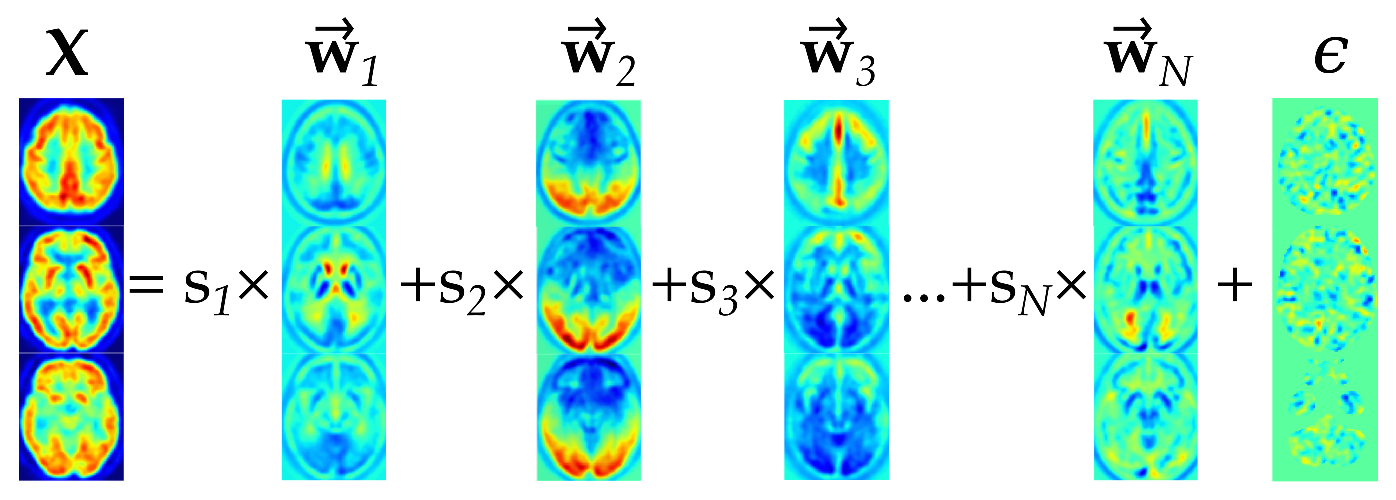
\includegraphics[width=\linewidth]{gfx/ch4/decomposition_overview}
	\caption[Illustration of how decomposition algorithms work.]{Illustration of how decomposition algorithms such as \ac{FA} and \ac{ICA} work on a \ac{PET}-FDG brain image.}
	\label{fig:decomposition_overview}
\end{figure}

Signal decomposition techniques are widely used in many applications, ranging from one-dimensional signals such as audio or Electroencephalography (EEG) to multidimensional arrays, and are frequently applied as feature reduction to overcome the small sample size problem, that is, the loss of statistical power due to a larger number of features compared to the number of samples. 

The pipeline that will be used throughout this chapter is displayed at Figure~\ref{fig:pipelineDecomposition}, involving a feature selection (for reducing the dimensionality), decomposition of the feature vectors and classification.
 
\begin{figure}[tph]
	\centering
	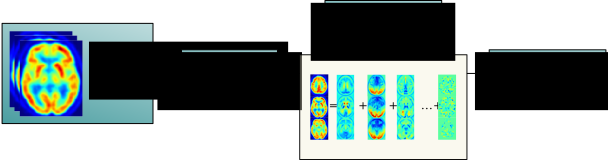
\includegraphics[width=\linewidth]{gfx/ch4/01-flowdiagram}
	\caption[Illustration of the system used in Chapter~\protect\ref{ch:decomposition} .]{Illustration of the system used in Chapter~\protect\ref{ch:decomposition}.}
	\label{fig:pipelineDecomposition}
\end{figure}

\section{Feature Selection}
Feature selection is the first strategy used for feature reduction [CITAR WILEY MIO], and it is often used along with feature extraction in order to build more complex pattern recognition systems. It refers to any strategy intended to find a subset of the original features containing the more suitable ones according to a certain criterion. Therefore, irrelevant features are discarded, and resultant models are faster and more cost-effective \cite{Guyon03}. However, it usually requires an additional optimization to find the parameters for the optimal feature subset, and furthermore, it is impossible to guarantee that the optimal features for the subset are the same of the full feature set \cite{DaelemansHosteMeulderEtAl2003}. 

In this work, we will use filtering methods to perform feature selection. Filtering methods are based on the computation of a feature relevance score directly on the data, before any interaction with the classification model. The relevance score is used to sort the different features, discarding those with a lower score, and it is usually computed independently for each feature, in what is called a univariate approach \cite{SaeysInzaLarranaga2007}. 

Explicar por qué usamos feature selection -> bajar tiempo de computación. 
\cite{Martinez201141,Martinez-Murcia20129676}

\subsection{$t$-Test}
Student's $t$-Test ($t$-Test) is a widely used statistical test which quantifies the differences between two different classes. It uses a common estimation of variance for both classes. The value of statistical $t$ can be computed \cite{Fay10} as: 

\begin{equation}
t = \frac{\bar {\Omega}_1 - \bar{\Omega}_2}{\sigma^2_{\Omega_1\Omega_2} \cdot \sqrt{\frac{1}{n_1}+\frac{1}{n_2}}}
\end{equation}
where
\begin{equation}
\sigma^2_{\Omega_1\Omega_2} = \sqrt{\frac{(n_1-1)\sigma^2_{\Omega_1}+(n_2-1)\sigma^2_{\Omega_2}}{n_1+n_2-2}}
\end{equation}
$\sigma^2_{\Omega_1 \Omega_2}$ is an estimator of common standard deviation of both samples, $\bar{\Omega}_1$ and $\bar{\Omega}_2$ are the mean of each class, $n_1$ is the number of samples in class $\omega_1$ and $n_2$ is the number of samples in class $\omega_2$. 

\subsection{Mann-Whitney-Wilcoxon} 
Mann-Whitney-Wilcoxon $U$-test(MWW) uses the absolute value of the statistical $U$ to rank voxels. Calculation of $U$ value is done by the following expression \cite{Fay10}:

\begin{equation}
U_i=R_i -  {n_i(n_i+1) \over 2} 
\end{equation}

\noindent where $n_i$ is the sample size for sample $i$, and $R_i$ is the sum of the ranks in sample $i$ (where $i=1,2$). Smaller $U_i$ value is taken as the final $U$ value. 

This statistical test measures the dissimilarity between two groups of values, and, although is similar to Student's t-Test, is less likely than it to spuriously indicate significance because of the presence of outliers. As we make use of real data, and we have no knowledge about the images' statistical distribution, MWW test could be a very good choice \cite{Fay10}.


\subsection{Relative Entropy} 
Relative Entropy (or Kullback-Leibler divergence) is a non-symmetric measure of the difference between two probability distributions $\Omega_1$ and $\Omega_2$. Because of its non-symmetric property, we can make use of this to evaluate the difference between CTRL and AD images for each voxel. Relative Entropy can be calculated with equation \ref{kullback} \cite{Theodoridis1999}. 

Let $\Omega_1$ and $\Omega_2$ be two discrete random variables. The Kullback-Leibler Divergence, or Relative Entropy is defined as:
\begin{equation}\label{kullback}
KL_{\omega_1 \omega_2} = \left(\frac{\sigma^2_2}{\sigma^2_1} +\frac{\sigma^2_1}{\sigma^2_2} -2 \right) + \frac{1}{2}\left(\mu_2-\mu_1\right)^2\left(\frac{1}{v_2} + \frac{1}{v_2}\right)
\end{equation}
where $\mu_c$ is the mean of class $c$, and $\sigma^2_c$ its variance. Figure \ref{fig:Zentropy} depicts values of Relative Entropy for each voxel. 

%klKL_{\omega_1 \omega_2} =  \int_{V} \omega_1 \log \frac{\omega_1}{\omega_2} \;d\mu
%\end{equation}
%\noindent where $\mu$ is any measure of $V$, the set of all voxels that are placed on a certain brain coordinate, in which $\omega_1 = \frac{d \Omega_1}{d \mu}$ and $\omega_2 = \frac{d \Omega_2}{d \mu}$ exist. Figure \ref{fig:Zentropy} depicts values of Relative Entropy for each voxel. 

\begin{figure}
	\centering
	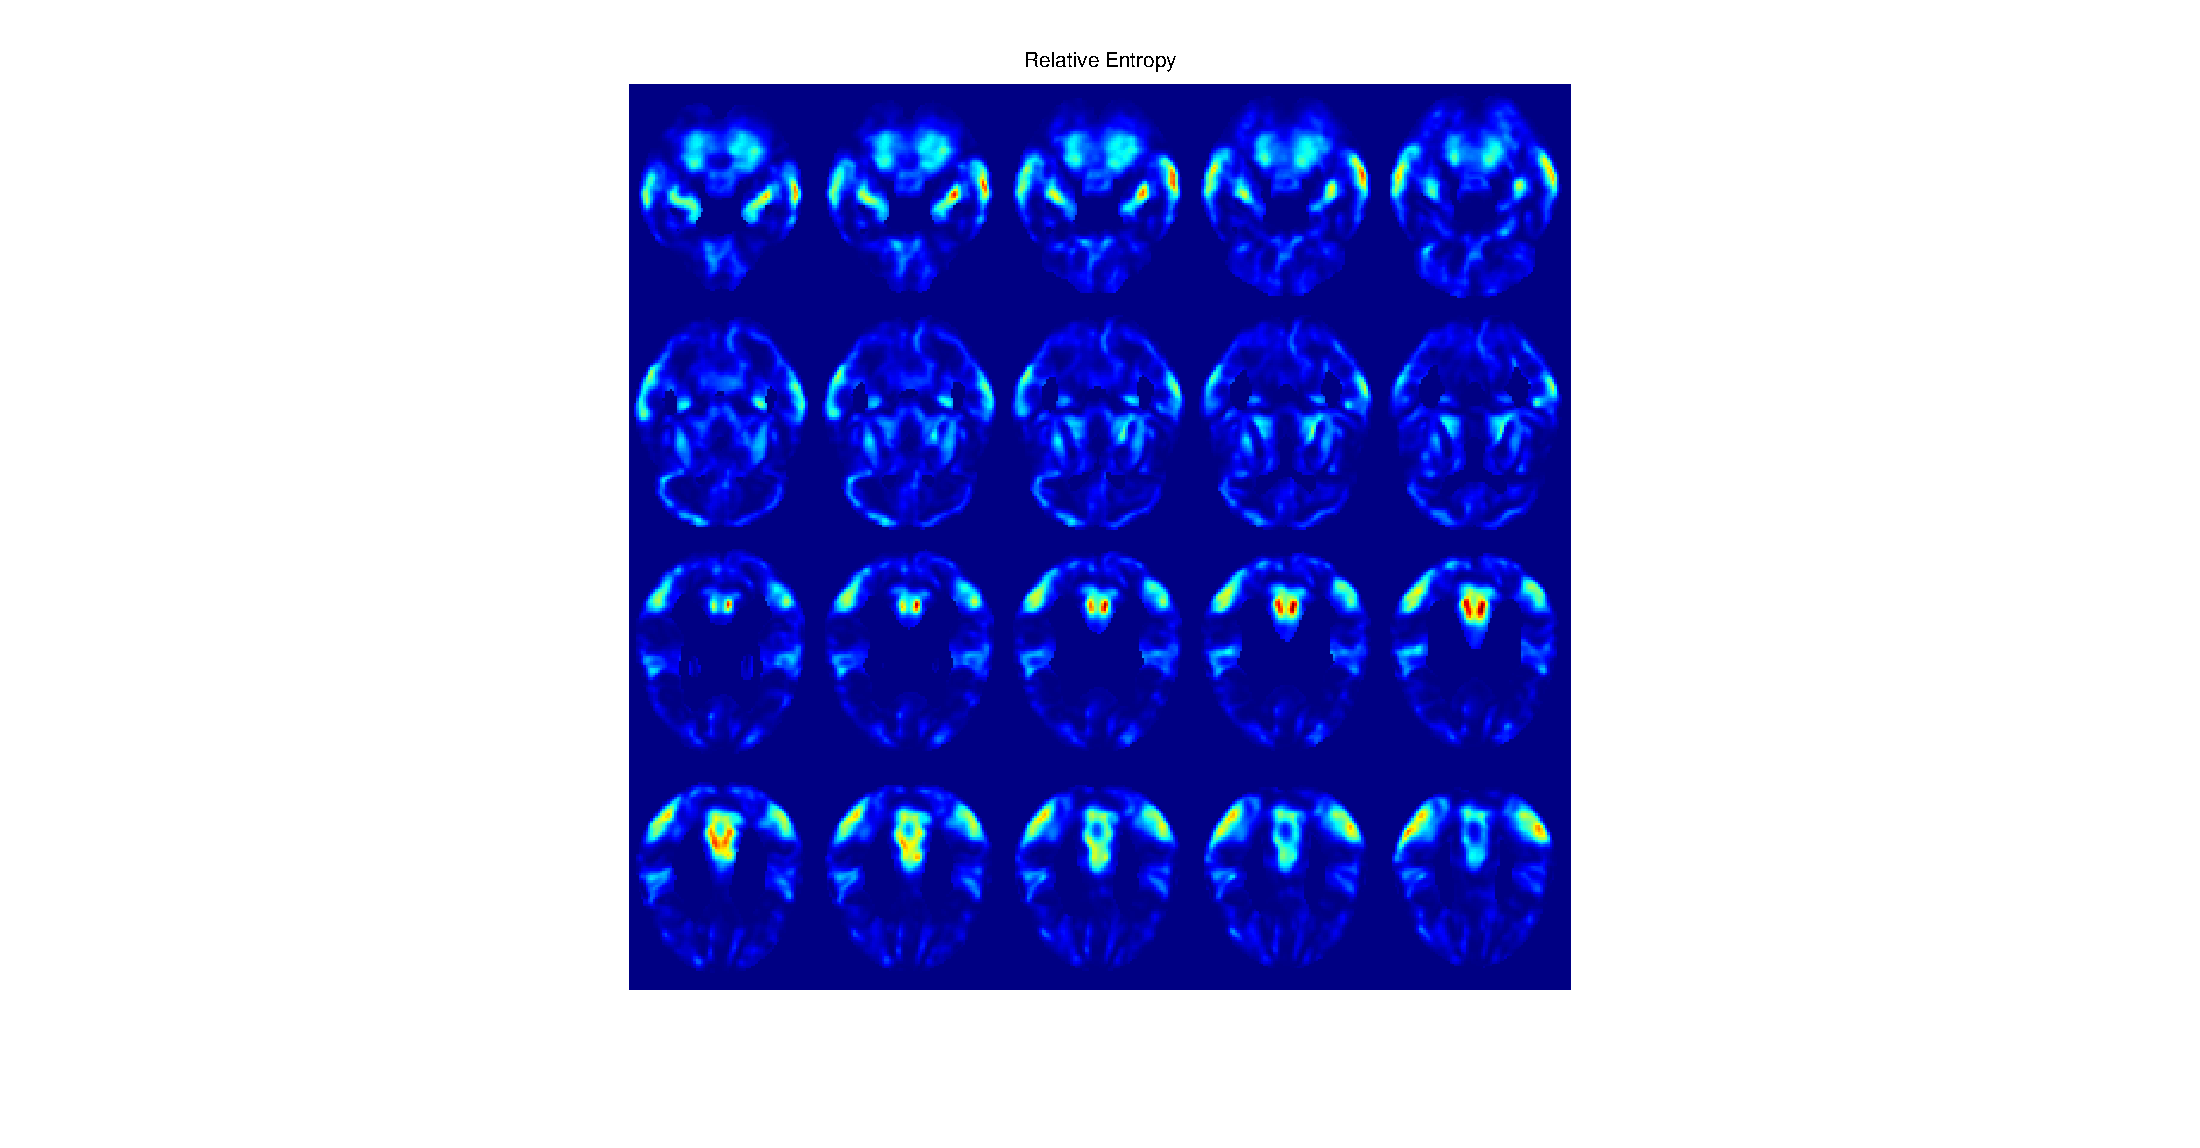
\includegraphics[width=0.7\linewidth]{gfx/ch4/Zentropy.eps}
	\caption{Several selected slices of the significance map obtained for each brain coordinate by applying the Relative Entropy criterium to the ADNI database.}
	\label{fig:Zentropy}
\end{figure}


\section{Decomposition Algorithms}
CITE WE WILL USE COMPONENT AND FACTOR INDEPENDENTLY. 
\subsection{Factor Analysis}
\cite{Martinez201141,Martinez-Murcia20129676}

To this purpose, a number of key features ($K$) are extracted using Fac\-tor A\-na\-ly\-sis technique \cite{Harman73}. It is assumed that each image in the database is a different observation of the experiment. Factor analysis models each of the $n$ observations as the expression of fewer unobserved variables, which are called factors. Each observation has $N$ variables, which are modelled as lineal combinations of the $K$ factors, plus errors, as described in Eq. \ref{eq:FactorAn1}.

\begin{equation}\label{eq:FactorAn1}
\textbf{x} = \mu + \boldsymbol\lambda \textbf{F} + \epsilon
\end{equation}

\noindent where \textbf{x} is the vector containing the observed variable (dimension $n$), $\mu$ is the mean of the variable, $\boldsymbol\lambda$ is a vector of $K$ factor loadings for this observation, $\textbf{F}$ is a matrix of dimension $N \times K$ which contains the common factors and $\epsilon$ is the error of reconstruction. For all observations, Eq. \ref{eq:FactorAn1} can be rewritted as:

\begin{equation}\label{eq:FactorAn2}
\textbf{X} = \boldsymbol\mu + \boldsymbol\Lambda \textbf{F} + \boldsymbol\epsilon
\end{equation}

\noindent where $\textbf{X}$ is a matrix of observed variables of dimension $n \times N$, $\boldsymbol\mu$ is a vector of means of length $n$, $\boldsymbol\Lambda$ is a matrix of dimension $n \times K$ which contains the maximum likelihood estimate of the factor loadings for each observation, $\textbf{F}$ is a matrix of dimension $N \times K$ which contains the common factors and $\boldsymbol\epsilon$ is a vector of length $n$ containing reconstruction errors.

\begin{figure*}[htp]
	\centering
	\begin{tabular}{cc}
		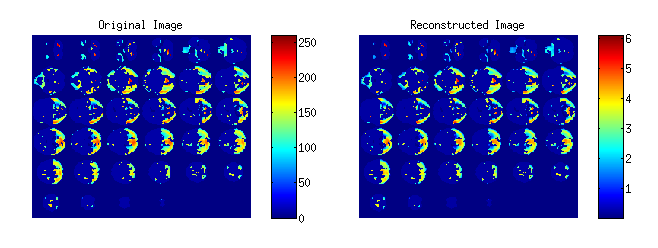
\includegraphics[width=\linewidth]{gfx/ch4/reconstruction}\\
	\end{tabular}
	\caption{\textit{a)} Original PET image composed by $N=7000$ selected voxels and \textit{b)} reconstruction using Factor Analysis with $K=13$ factors extracted.}
	\label{fig:reconstruction}
\end{figure*}

Original input image can be reconstructed with computed factors and factor loadings, as we have seen in Eq. \ref{eq:FactorAn1}. In Fig. \ref{fig:reconstruction} original image and Factor Analysis reconstruction are shown. The selected regions pinpoint the disease affected areas which are class-discriminative. Specifically, it highlights the posterior cingulate gyri and precunei, as well as the temporo-parietal region, both considered as typically affected by glucose hypometabolism in the AD \cite{Claus1994}. A closer look shows that it also selects small thalamus regions, which has never been described as a relevant region for diagnosis. To compute representativeness of different factors, we can rewrite Eq. \ref{eq:FactorAn2} as:

\begin{equation}\label{eq:cov}
Cov (\textbf{X} - \boldsymbol\mu) = Cov(\boldsymbol\Lambda \textbf{F} - \boldsymbol\epsilon)
\end{equation}

If $\Sigma$ stands for $Cov (\textbf{X} - \boldsymbol\mu)$, Eq. \ref{eq:cov} can be rewritted as:

\begin{equation}
\boldsymbol\Sigma = \boldsymbol\Lambda Cov(\textbf{F}) \boldsymbol\Lambda^T - Cov(\boldsymbol\epsilon)
\end{equation}

\begin{equation}
\boldsymbol\Sigma = \boldsymbol\Lambda \boldsymbol\Lambda^T - \boldsymbol\Psi
\end{equation}

\noindent and extract $\Psi$, the diagonal matrix containing the specific variances of the reconstruction error.

The choice of K requires a deeper analysis. If $K$ is large, the image can be modelled very well, and therefore, the reconstruction error should be small. However, a large number of features can be counter-productive for the performance of the classifier due to the small sample size problem. Thus, we should find a trade-off between the length of the feature vectors ($K$) and the ability of reconstruction. According to Fig. \ref{fig:error}, the variance reconstruction error tends to stabilize as $K$ increases, and the improvements are no longer significant. In the experimental Section \ref{results} a detailed discussion about $K$ parameter selection is shown in addition with other experimental findings.

\begin{figure}[ht]
	\centering
	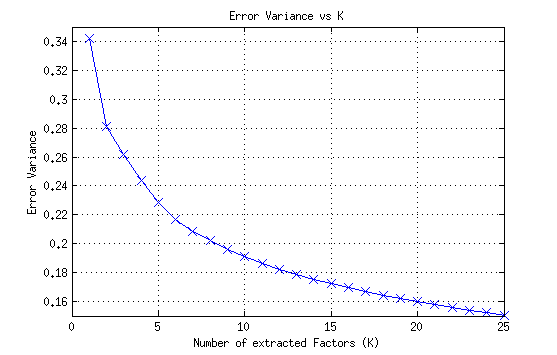
\includegraphics[width=0.45\linewidth]{gfx/ch4/varError-K-ADNI}
	\caption{Specific variance of reconstruction error $\Psi$ using Factor Analysis, in function of number of factors extracted ($K$) for ADNI database (the behaviour is similar in other datasets).}
	\label{fig:error}
\end{figure}

\subsection{Independent Component Analysis}
\cite{Martinez-Murcia2013255,Martinez-Murcia201458}

\acf{ICA} \cite{Hyvarinen2000}, is a statistical technique that represents a multidimensional random vector as a lineal combination of non-gaussian random variables (the so-called ''independent components'') to be as independent as possible, and has been used widely on segmentation and clustering of medical images \cite{DeMartino2007,Alvarez2009}. It can be considered as a non-gaussian version of Factor Analysis. Assume that we observe $n$ lineal mixtures $\mathbf{x}_1, \mathbf{x}_2, \ldots, \mathbf{x}_n$ of length $N$ that can be modelled as an expression of $K$ independent components (IC). These independent components are defined as $\mathbf{S} = (\mathbf{s}_1, \mathbf{s}_2, ... \mathbf{s}_K)$, where each $\mathbf{s}_K$ vector has a length of $N$. So, each random vector $\mathbf{x}_n$ can be described as a linear combination of $K$ independent components: 

\begin{equation}
\mathbf{x_n} = a_{1n}\mathbf{s}_1 + a_{2n}\mathbf{s}_2 + \ldots + a_{Kn}\mathbf{s}_K
\end{equation}

Without loss of generality we can assume that both the observed vectors and the independent components are are zero mean. If the previous conditions are not met, the $\mathbf{x}$ variables can be centered by subtracting the sample mean. To use a vector-matrix notation, more convenient in this case, we denote as matrix $\mathbf{X}$ the random vector whose elements are $\mathbf{x}_1, \ldots, \mathbf{x}_n$. We also denote as $\mathbf{A}$ the matrix that contains all $a_{Kn}$ elements, the ''mixing matrix'' that projects each image into the space defined by the IC. Using this notation, the mixing model above remains as follows: 

\begin{equation}\label{eq:ica}
\mathbf{X}=\mathbf{A}\mathbf{S}
\end{equation}

The starting point of ICA is the assumption that all components $\mathbf{s}_K$ are are statistically independent. To measure independence, we assume that all independent components have a non-gaussian statistical distribution. It is assumed that a sum of independent signal trends to gaussianity, so if non-gaussianity is maximized with any independence criteria $F$, for instance, the kurtosis or negentropy, we obtain signals that are more independent than the previous ones \cite{Hyvarinen1999,Hyvarinen2000}.
After estimating the matrix $\mathbf{A}$, we can compute its inverse, $\mathbf{W}$ and obtain the projection $\mathbf{S}$ of the images in the dataset into the IC space with: 
\begin{equation}
\mathbf{S} = \mathbf{W}\mathbf{X}
\end{equation}

\subsubsection{FastICA}
Adaptive algorithms based on gradient descend can be problematic when they are used on an environment in which adaptation is not necessary, like this case. The convergence is often slow, and depends on the choice of convergence parameters. As a solution to this problem, block algorithms based on fixed-point iteration \cite{Oja1997,FastICA99} can be used. In \cite{Oja1997} a fixed-point algorithm based on kurtosis is introduced. In \cite{FastICA99}, this algorithm, known as FastICA, is generalized to general contrast functions. The single unit FastICA algorithm has the following form:
\begin{equation}
\mathbf{w}(k) = E\lbrace\mathbf{x}g(\mathbf{w}(k-1)^T\mathbf{x})\rbrace -E\lbrace g'(\mathbf{w}(k-1)^T\mathbf{x})\rbrace\mathbf{w}(k-1)
\end{equation}
where the loadings vector $\mathbf{w}$ is normalized to unit norm in each iteration, and the function $g(x)$ is a derivative of the contrast function $G$ defined in \cite{Hyvarinen1999}. The expected values are estimated in practice by using the mean of a significantly high number of samples of the input data. 
The speed of convergence of the fixed-point algorithms is clearly superior to more neural algorithms. Improvements between 10 and 100 times the speed are observed frequently \cite{Giannakopoulos1998}. 


% AQUÍ EMPIEZA LO QUE HEMOS ESCRITO YA. 
\section{Results}
In this work we will analyse the behaviour of the system proposed in the introduction and illustrated at Figure~\ref{fig:pipelineDecomposition}. The system comprises the selection of the most relevant voxels using filtering methods (we will focus on $t$-test, relative entropy and wilcoxon) and a feature decomposition of these using either \ac{FA} or \ac{ICA}. Finally, the feature vectors are classified using a \ac{SVC} with linear kernel, and performance values are obtained via cross-validation (see Section~\ref{sec:validation} for more information). 

We vary the number of selected voxels and the number of factors or components depending on the algorithm and the dataset used and evaluate the system with those characteristics. That way, we obtain an estimation of the performance of the system in different situations, so that we can draw conclusions on the disease patterns and the ability of the system in the detection of different diseases. 

\subsection{Alzheimer's Disease}
We begin by applying the proposed feature selection plus decomposition pipeline to the two functional neuroimaging datasets: ADNI-PET and VDLN-HMPAO. For this experiment we will use a maximum of $20,000$ selected voxels and $25$ components. 

\subsubsection{Factor Analysis}\label{sec:results_FA_AD}
First, we use \ac{FA} as a decomposition technique. In Figure~\ref{fig:accuracyMeanFA-AD} we average the accuracy over the number of voxels or the number of components respectively, to look at how these variables affect the performance of the system, and we do this for the three filtering methods used. 

\begin{bigfigure}[-2cm]
	\centering
	\subfloat[]{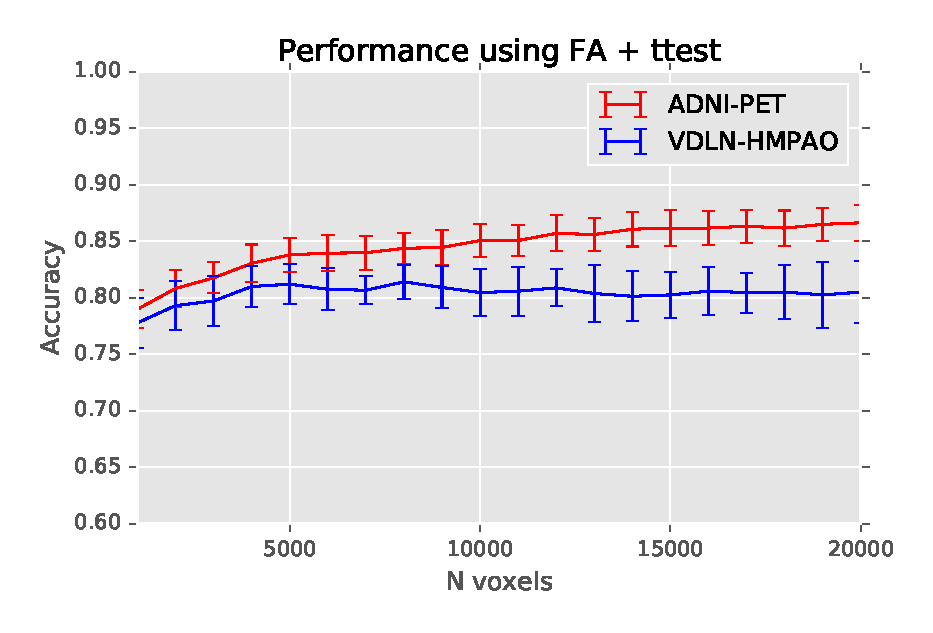
\includegraphics[width=0.49\linewidth]{gfx/ch4/accuracyMeanSTD-FA_vsN_ttest_AD.eps}\label{fig:AD-AV-FA-TTEST-VSN}}
	\subfloat[]{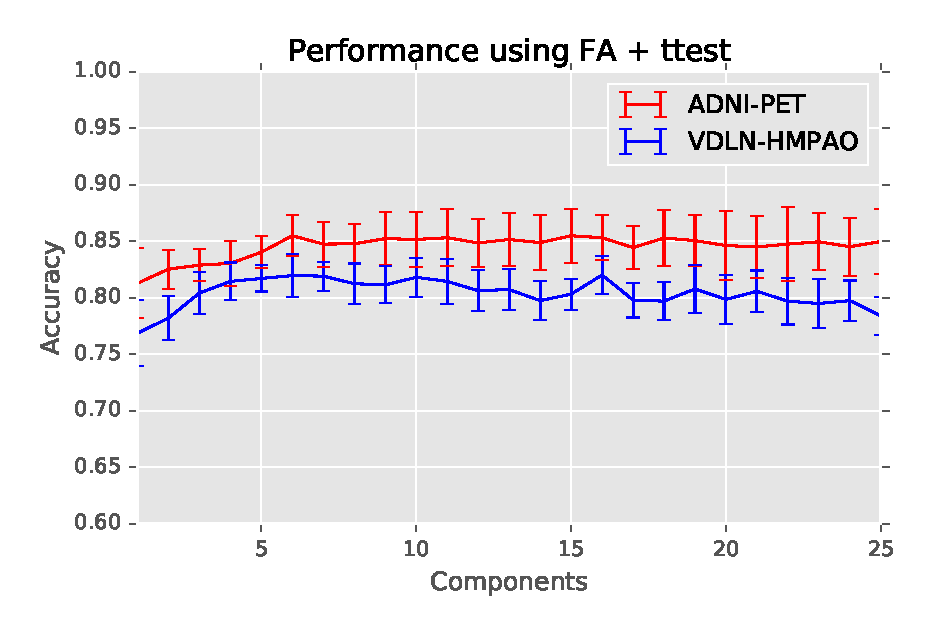
\includegraphics[width=0.49\linewidth]{gfx/ch4/accuracyMeanSTD-FA_vsK_ttest_AD.eps}\label{fig:AD-AV-FA-TTEST-VSK}}
	
	\subfloat[]{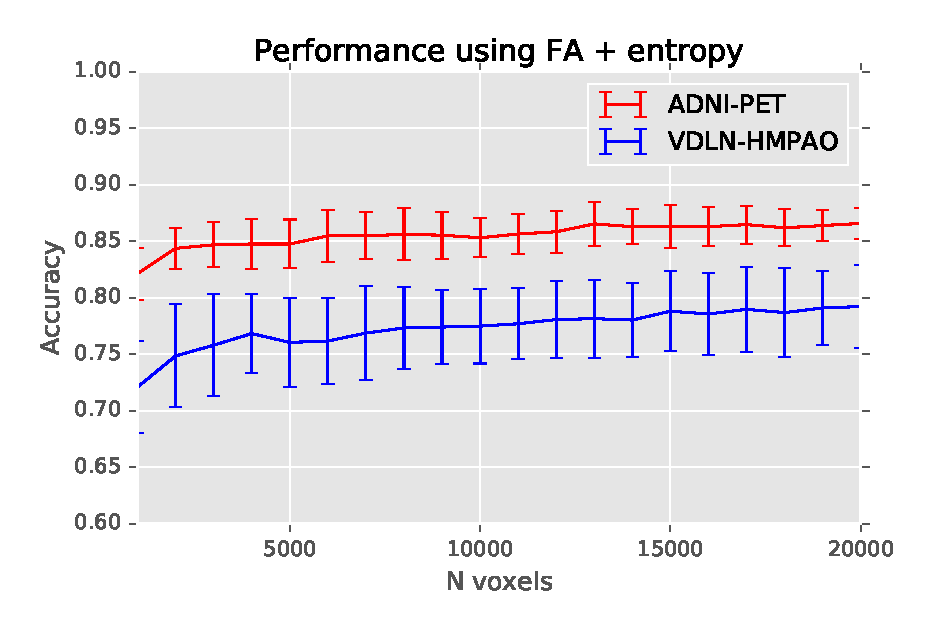
\includegraphics[width=0.49\linewidth]{gfx/ch4/accuracyMeanSTD-FA_vsN_entropy_AD.eps}\label{fig:AD-AV-FA-ENTROPY-VSN}}
	\subfloat[]{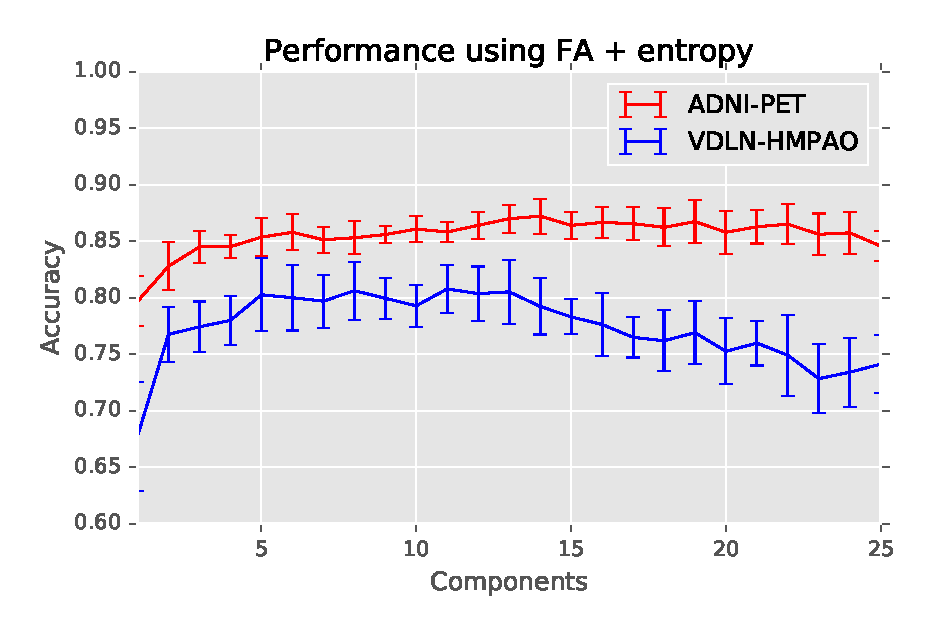
\includegraphics[width=0.49\linewidth]{gfx/ch4/accuracyMeanSTD-FA_vsK_entropy_AD.eps}\label{fig:AD-AV-FA-ENTROPY-VSK}}
	
	\subfloat[]{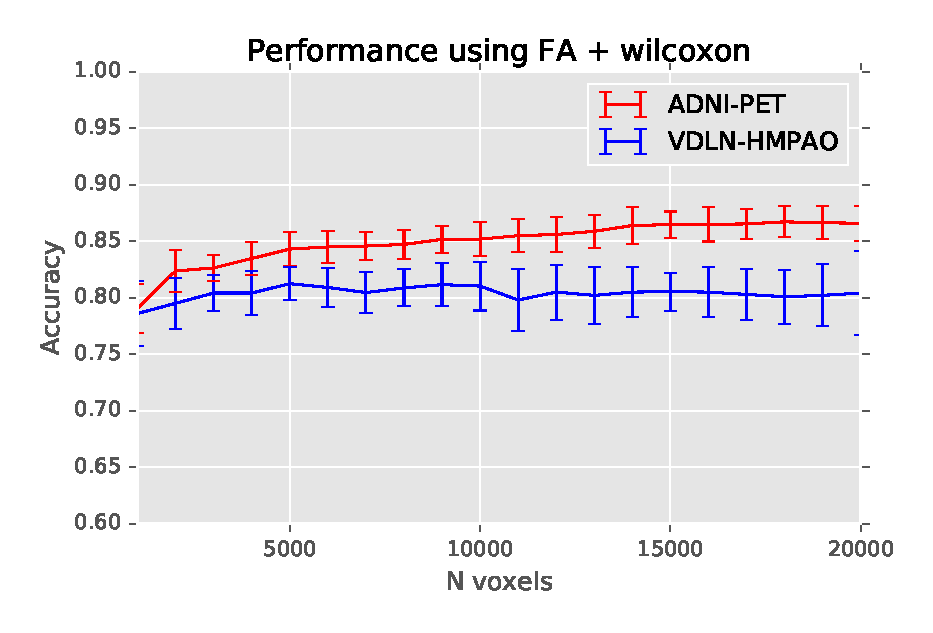
\includegraphics[width=0.49\linewidth]{gfx/ch4/accuracyMeanSTD-FA_vsN_wilcoxon_AD.eps}\label{fig:AD-AV-FA-WILCOXON-VSN}}
	\subfloat[]{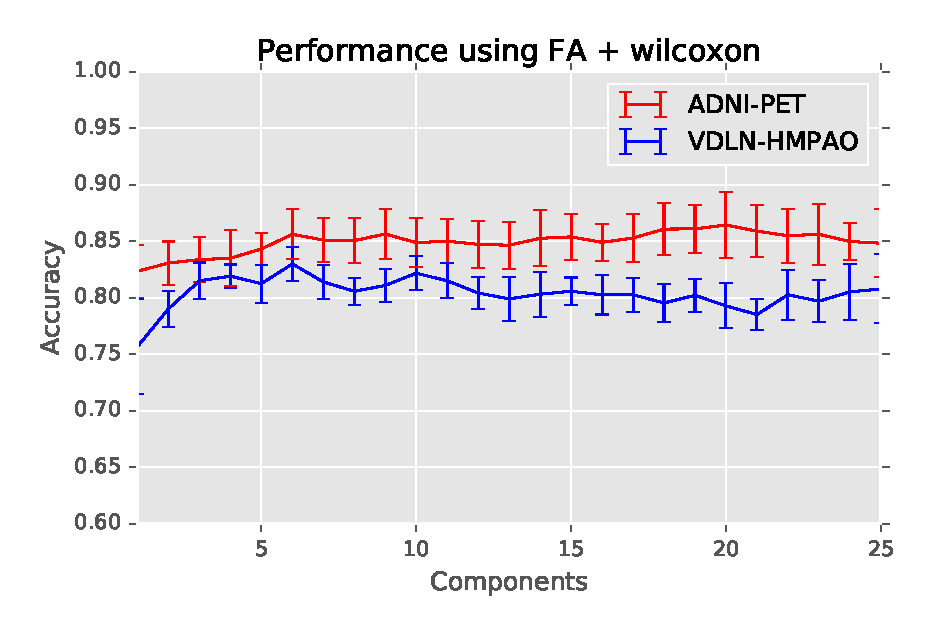
\includegraphics[width=0.49\linewidth]{gfx/ch4/accuracyMeanSTD-FA_vsK_wilcoxon_AD.eps}\label{fig:AD-AV-FA-WILCOXON-VSK}}
	
	\caption{Average performance and standard deviation of the proposed system using the two \ac{AD} datasets, \ac{FA} and the three feature selection criteria: $t$-test (\protect\subref{fig:AD-AV-FA-TTEST-VSN} and \protect\subref{fig:AD-AV-FA-TTEST-VSK}), relative entropy (\protect\subref{fig:PKS-AV-FA-ENTROPY-VSN} and \protect\subref{fig:AD-AV-FA-ENTROPY-VSK}) and wilcoxon (\protect\subref{fig:AD-AV-FA-WILCOXON-VSN} and \protect\subref{fig:AD-AV-FA-WILCOXON-VSK}). } 
	\label{fig:accuracyMeanFA-AD}
\end{bigfigure}

We can observe that the results are always better when using the ADNI-PET dataset than with the VDLN-HMPAO, and this is especially notorious when using the relative entropy selection criterion. The performance tends to slightly increase with the number of voxels selected, but it is not the case with the number of components. By looking at figures \ref{fig:AD-AV-FA-TTEST-VSK}, \ref{fig:AD-AV-FA-ENTROPY-VSK} and \ref{fig:AD-AV-FA-WILCOXON-VSK}, it seems that a relatively small number of components (approximately 6) is enough to obtain good performance, and afterwards, the performance holds or even decreases. 

\subsubsection{Independent Component Analysis}
In this section, we compute the results of applying \ac{ICA} to the ADNI-PET and VDLN-HMPAO datasets. Figure~\ref{fig:accuracyMeanICA-AD} depicts the average accuracy over the number of voxels or the number of components respectively for the different selection criteria. 

\begin{bigfigure}[-2cm]
	\centering
	\subfloat[]{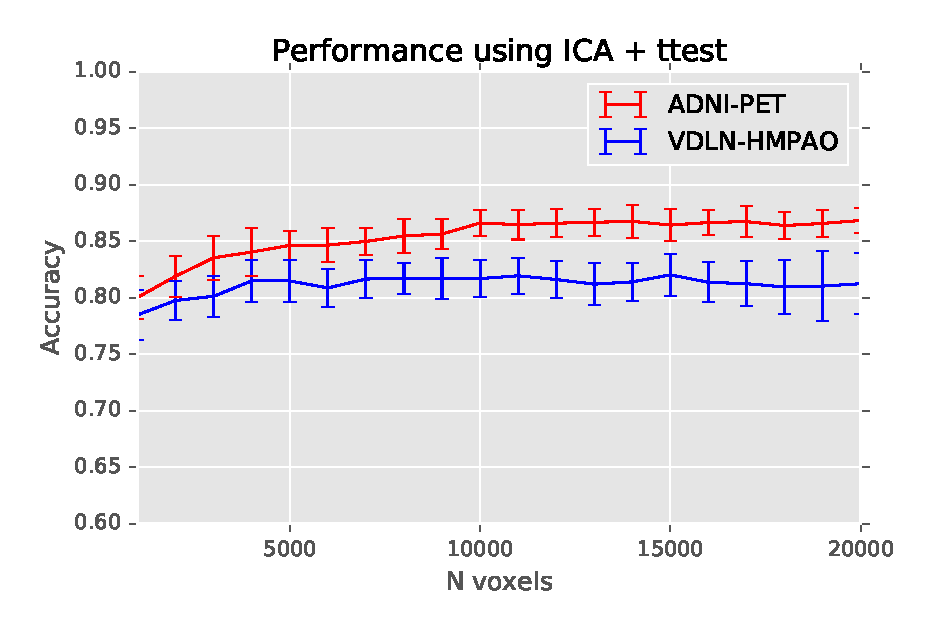
\includegraphics[width=0.49\linewidth]{gfx/ch4/accuracyMeanSTD-ICA_vsN_ttest_AD.eps}\label{fig:AD-AV-ICA-TTEST-VSN}}
	\subfloat[]{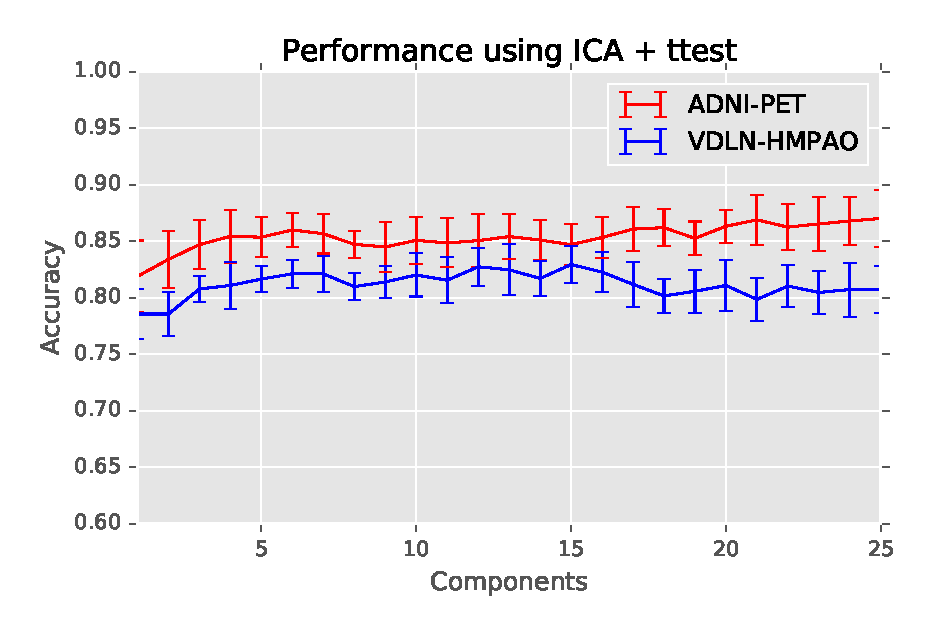
\includegraphics[width=0.49\linewidth]{gfx/ch4/accuracyMeanSTD-ICA_vsK_ttest_AD.eps}\label{fig:AD-AV-ICA-TTEST-VSK}}
	
	\subfloat[]{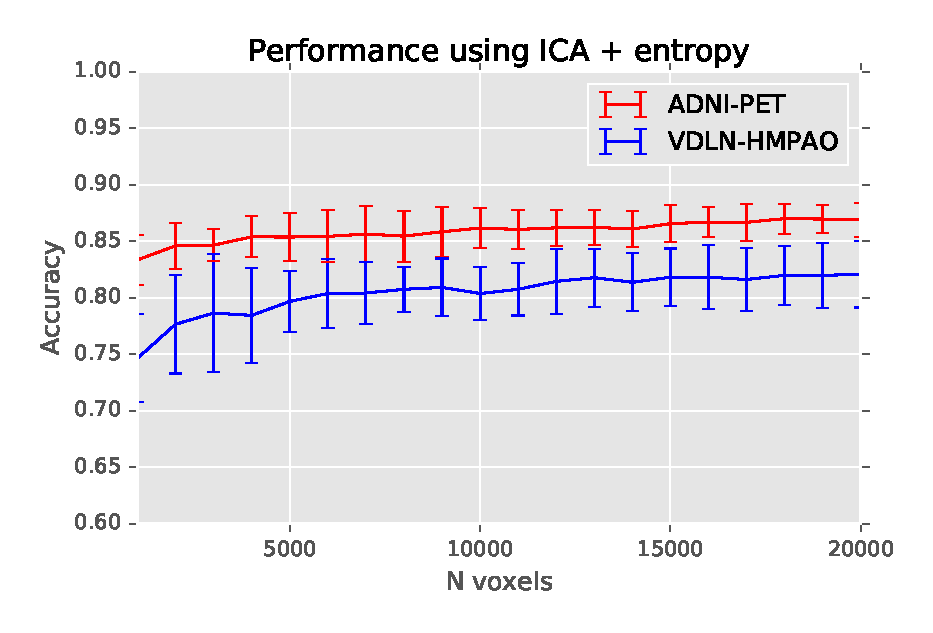
\includegraphics[width=0.49\linewidth]{gfx/ch4/accuracyMeanSTD-ICA_vsN_entropy_AD.eps}\label{fig:AD-AV-ICA-ENTROPY-VSN}}
	\subfloat[]{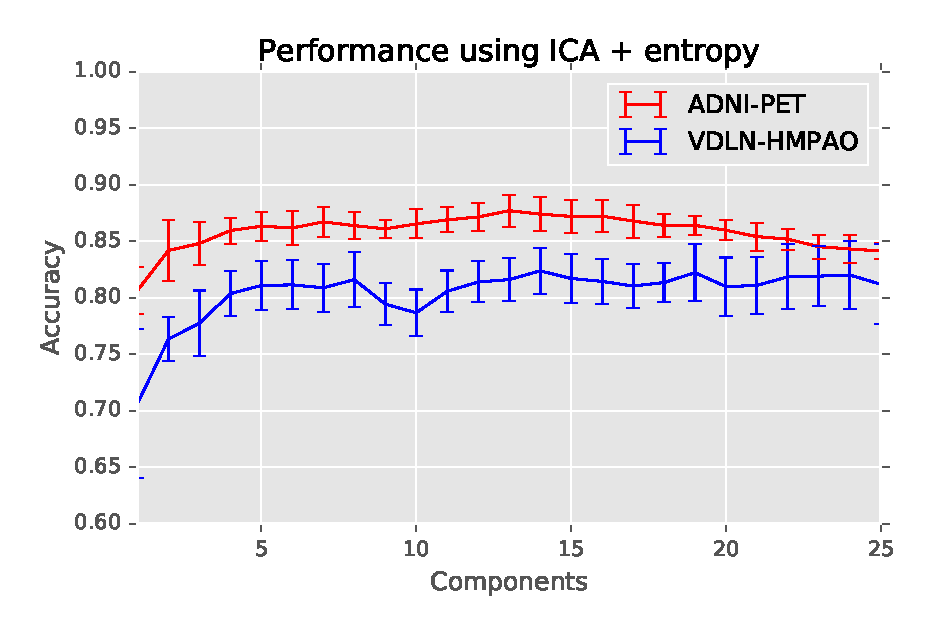
\includegraphics[width=0.49\linewidth]{gfx/ch4/accuracyMeanSTD-ICA_vsK_entropy_AD.eps}\label{fig:AD-AV-ICA-ENTROPY-VSK}}
	
	\subfloat[]{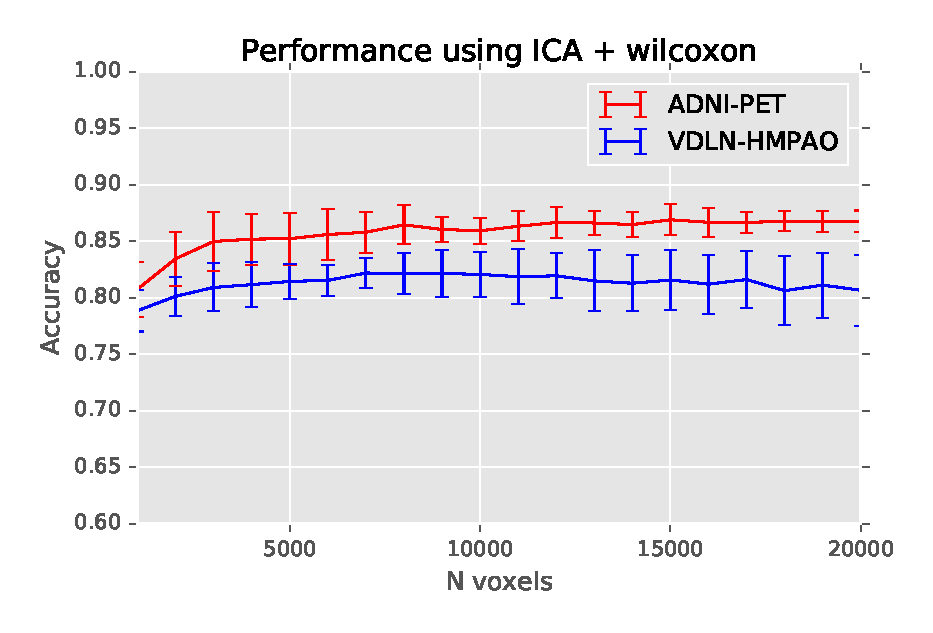
\includegraphics[width=0.49\linewidth]{gfx/ch4/accuracyMeanSTD-ICA_vsN_wilcoxon_AD.eps}\label{fig:AD-AV-ICA-WILCOXON-VSN}}
	\subfloat[]{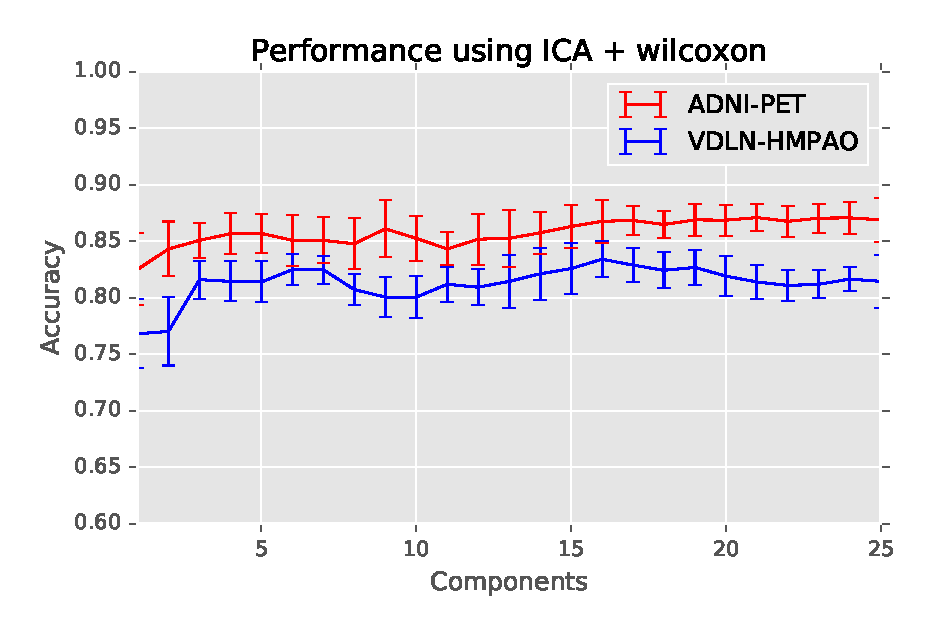
\includegraphics[width=0.49\linewidth]{gfx/ch4/accuracyMeanSTD-ICA_vsK_wilcoxon_AD.eps}\label{fig:AD-AV-ICA-WILCOXON-VSK}}
	
	\caption{Average performance and standard deviation of the proposed system using the three \ac{AD} datasets, \ac{ICA} and the three feature selection criteria: $t$-test (\protect\subref{fig:AD-AV-ICA-TTEST-VSN} and \protect\subref{fig:AD-AV-ICA-TTEST-VSK}), relative entropy (\protect\subref{fig:AD-AV-ICA-ENTROPY-VSN} and \protect\subref{fig:AD-AV-ICA-ENTROPY-VSK}) and wilcoxon (\protect\subref{fig:AD-AV-ICA-WILCOXON-VSN} and \protect\subref{fig:AD-AV-ICA-WILCOXON-VSK}). } 
	\label{fig:accuracyMeanICA-AD}
\end{bigfigure}

The case is similar to the one presented in Section~\ref{sec:results_FA_AD}, where the performance slightly improves when increasing the number of selected voxels. The performance is again better when using the ADNI-PET dataset than with the VDLN-HMPAO, although the behaviour is similar. 

The results change when varying the number of components. In this case, although good performance is obtained within the first 5 components in most cases, the performance does not decrease with a higher number, and sometimes increases (for example, in the case of \ac{ICA} and the $t$-test or the wilcoxon selection criteria). 

\subsubsection{At the Operation Point}
Now we focus on non-averaged values, the values for which our system is optimal: the operation point. 

\begin{bigfigure}[-2cm]
	\centering
	\subfloat[]{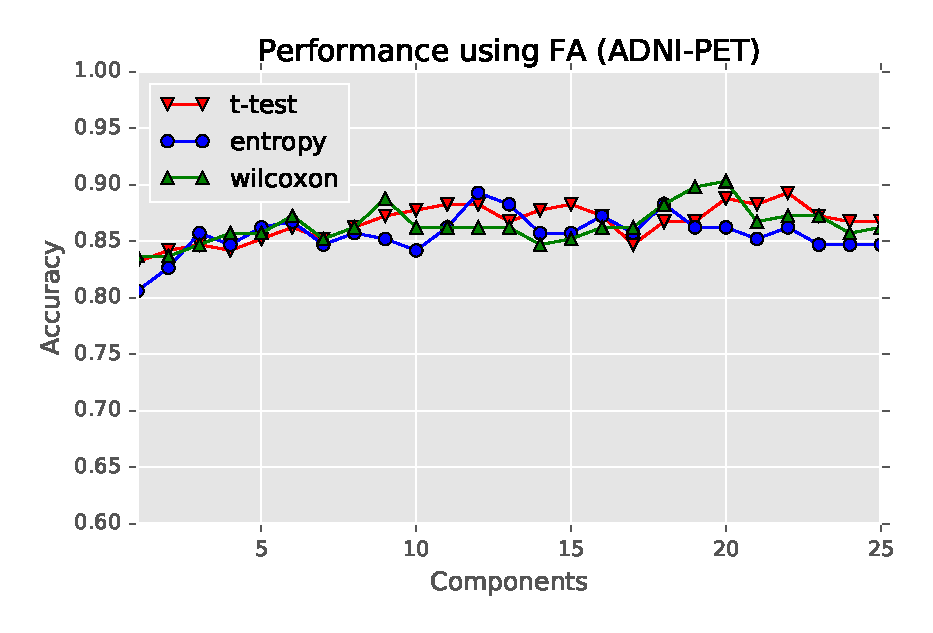
\includegraphics[width=0.49\linewidth]{gfx/ch4/accuracyOP-FA_vsN_comparison_ADNI-PET.eps}\label{fig:ADNI-PET-FA-OP}}
	\subfloat[]{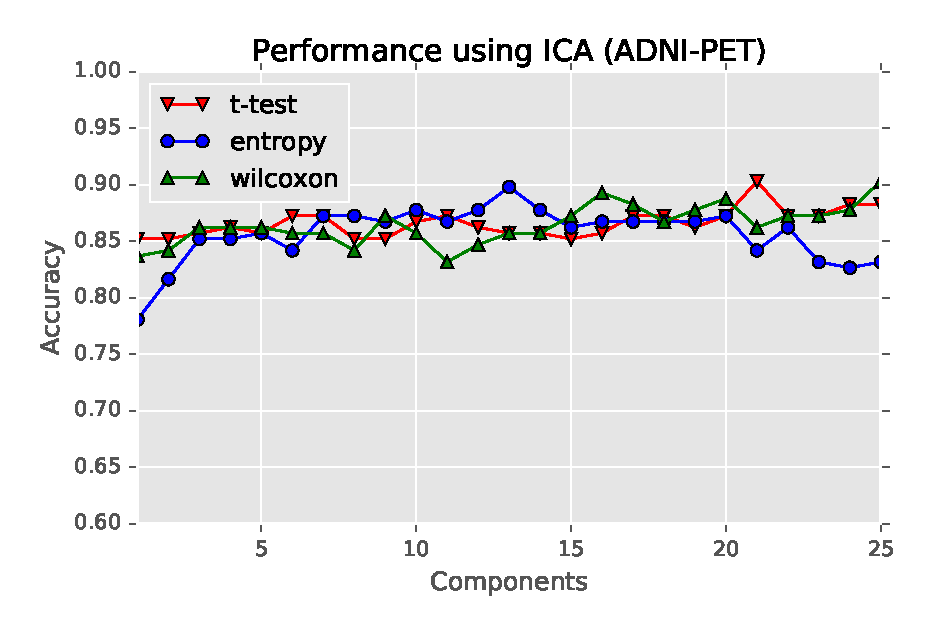
\includegraphics[width=0.49\linewidth]{gfx/ch4/accuracyOP-ICA_vsN_comparison_ADNI-PET.eps}\label{fig:ADNI-PET-ICA-OP}}
	
	\subfloat[]{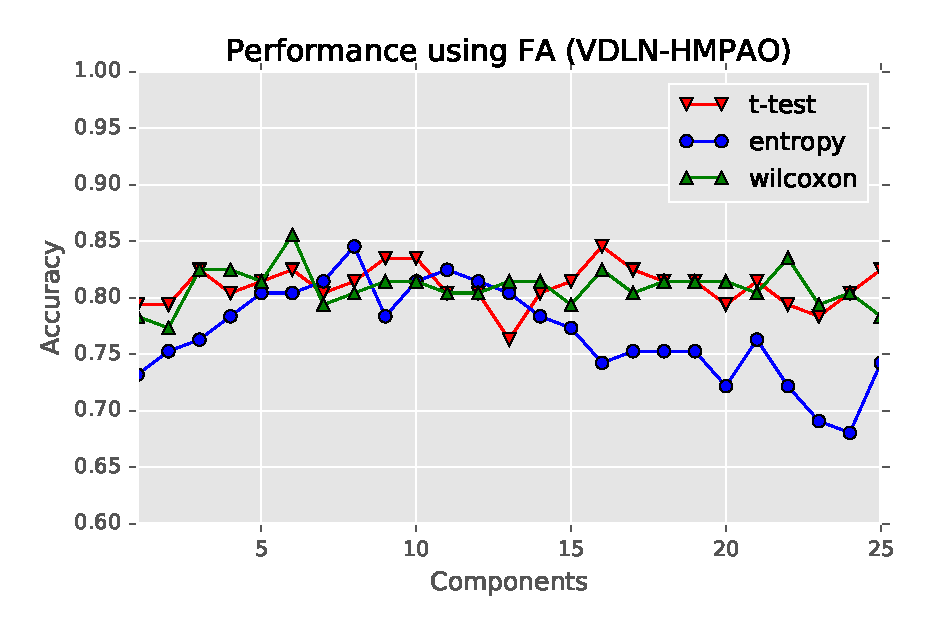
\includegraphics[width=0.49\linewidth]{gfx/ch4/accuracyOP-FA_vsN_comparison_VDLN-HMPAO.eps}\label{fig:VDLN-HMPAO-FA-OP}}
	\subfloat[]{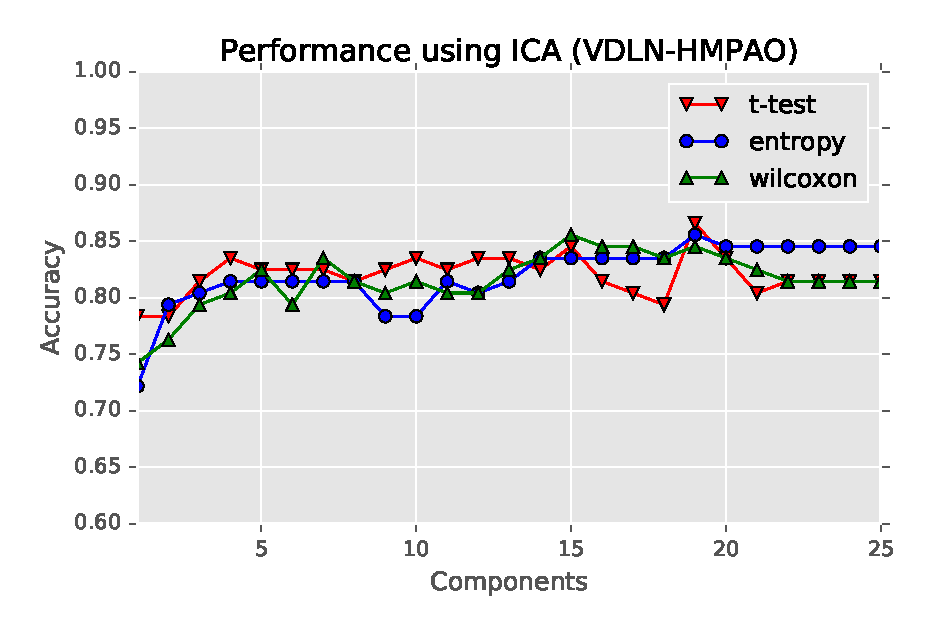
\includegraphics[width=0.49\linewidth]{gfx/ch4/accuracyOP-ICA_vsN_comparison_VDLN-HMPAO.eps}\label{fig:VDLN-HMPAO-ICA-OP}}
	
	\caption{Performance of the proposed system using the two \ac{AD} datasets: ADNI-PET and VDLN-HMPAO at the operation point, and how they vary over the number of components used in the decomposition. } 
	\label{fig:accuracyOP-AD}
\end{bigfigure}


\begin{bigtable}[-2cm]
	\begin{tabularx}{\linewidth}{Xllccc}
		\tableheadline{DB} & \tableheadline{Dec.} & \tableheadline{Criterion} & \tableheadline{Accuracy} & \tableheadline{Sensitivity} & \tableheadline{Specificity}\\
		\toprule
		\multirow{6}{1.7cm}{ADNI- PET} & \multirow{3}{*}{\ac{FA}} & t-test & $ 0.893 \pm 0.074 $ & $ 0.886 \pm 0.119 $ & $ 0.901 \pm 0.101 $ \\
		&  & entropy & $ 0.893 \pm 0.074 $ & $ 0.894 \pm 0.092 $ & $ 0.891 \pm 0.088 $ \\
		&  & wilcoxon & $ 0.903 \pm 0.066 $ & $ 0.917 \pm 0.079 $ & $ 0.891 \pm 0.082 $ \\
		\cline{2-6}
		& \multirow{3}{*}{\ac{ICA}} & t-test & $ 0.903 \pm 0.071 $ & $ 0.893 \pm 0.100 $ & $ 0.910 \pm 0.107 $ \\
		&  & entropy & $ 0.898 \pm 0.059 $ & $ 0.917 \pm 0.088 $ & $ 0.881 \pm 0.084 $ \\
		&  & wilcoxon & $ 0.903 \pm 0.066 $ & $ 0.906 \pm 0.097 $ & $ 0.901 \pm 0.094 $ \\ \midrule
		\multirow{6}{1.7cm}{VDLN- HMPAO} & \multirow{3}{*}{\ac{FA}} & t-test & $ 0.845 \pm 0.102 $ & $ 0.843 \pm 0.158 $ & $ 0.855 \pm 0.140 $ \\
		&  & entropy & $ 0.845 \pm 0.052 $ & $ 0.893 \pm 0.146 $ & $ 0.785 \pm 0.163 $ \\
		&  & wilcoxon & $ 0.856 \pm 0.084 $ & $ 0.857 \pm 0.137 $ & $ 0.855 \pm 0.151 $ \\
		\cline{2-6}
		& \multirow{3}{*}{\ac{ICA}} & t-test & $ 0.866 \pm 0.085 $ & $ 0.873 \pm 0.144 $ & $ 0.855 \pm 0.154 $ \\
		&  & entropy & $ 0.856 \pm 0.101 $ & $ 0.853 \pm 0.138 $ & $ 0.855 \pm 0.151 $ \\
		&  & wilcoxon & $ 0.856 \pm 0.086 $ & $ 0.857 \pm 0.156 $ & $ 0.855 \pm 0.160 $ \\
		\bottomrule
	\end{tabularx}
	\caption{Accuracy, sensitivity, specificity, and their standard deviation at the operation point for each method and its corresponding feature selection criterion, using two \protect\ac{AD} datasets. }
	\label{tab:featureAD}
\end{bigtable}
\FloatBarrier
\subsection{Parkinson's Disease}


\subsubsection{Factor Analysis}
\begin{bigfigure}[-2cm]
	\centering
	\subfloat[]{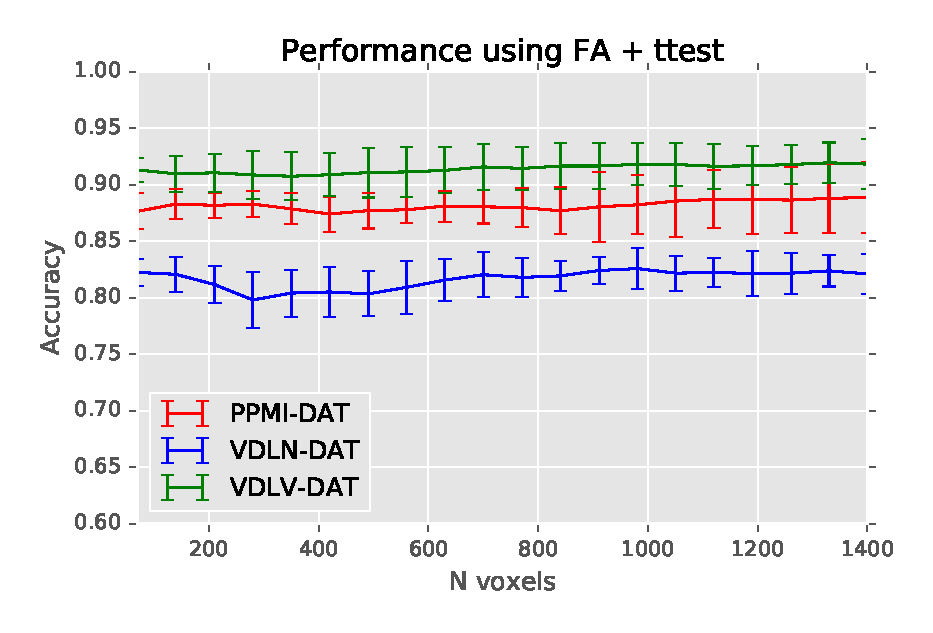
\includegraphics[width=0.49\linewidth]{gfx/ch4/accuracyMeanSTD-FA_vsN_ttest_PKS.eps}\label{fig:PKS-AV-FA-TTEST-VSN}}
	\subfloat[]{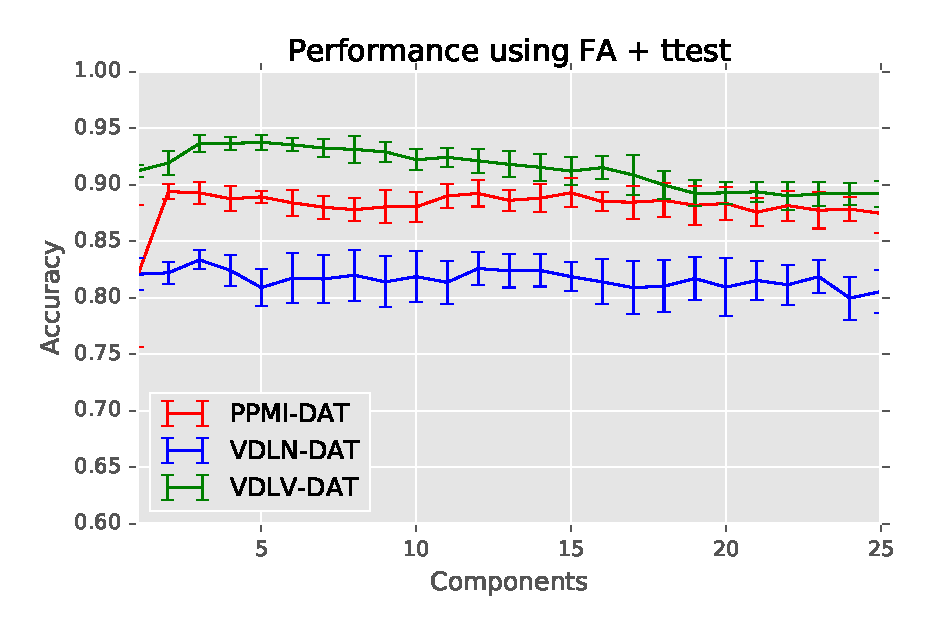
\includegraphics[width=0.49\linewidth]{gfx/ch4/accuracyMeanSTD-FA_vsK_ttest_PKS.eps}\label{fig:PKS-AV-FA-TTEST-VSK}}
	
	\subfloat[]{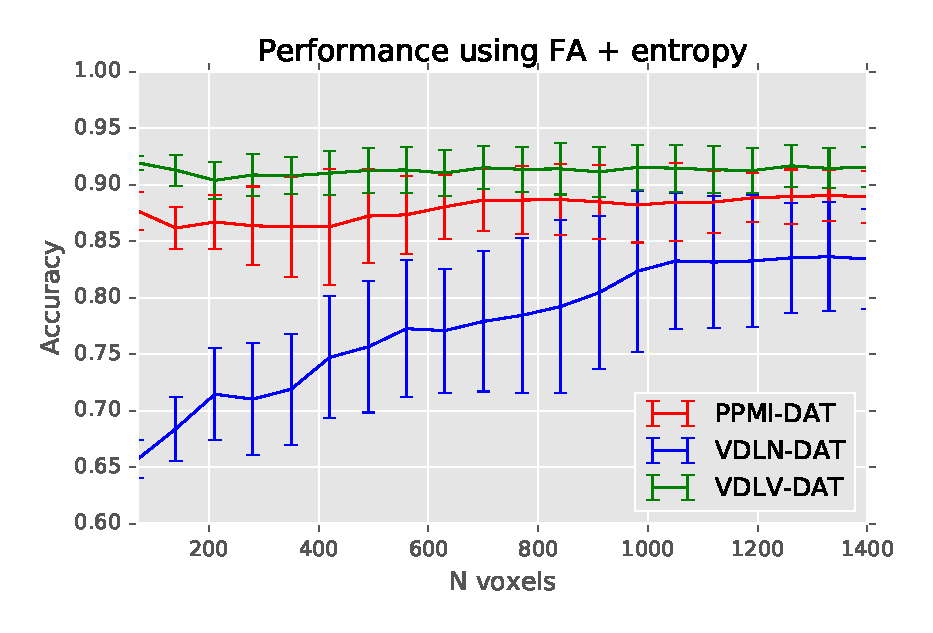
\includegraphics[width=0.49\linewidth]{gfx/ch4/accuracyMeanSTD-FA_vsN_entropy_PKS.eps}\label{fig:PKS-AV-FA-ENTROPY-VSN}}
	\subfloat[]{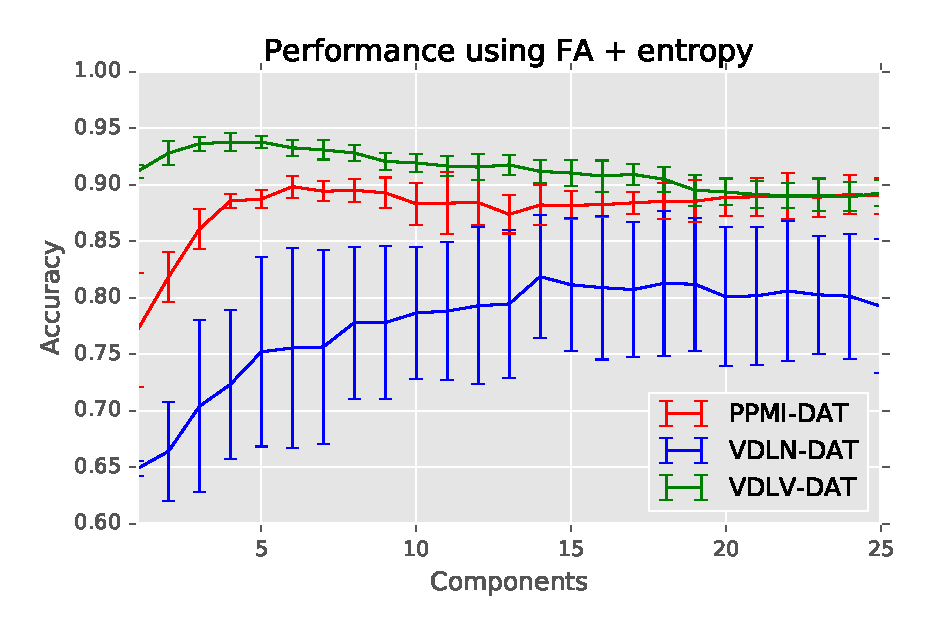
\includegraphics[width=0.49\linewidth]{gfx/ch4/accuracyMeanSTD-FA_vsK_entropy_PKS.eps}\label{fig:PKS-AV-FA-ENTROPY-VSK}}
	
	\subfloat[]{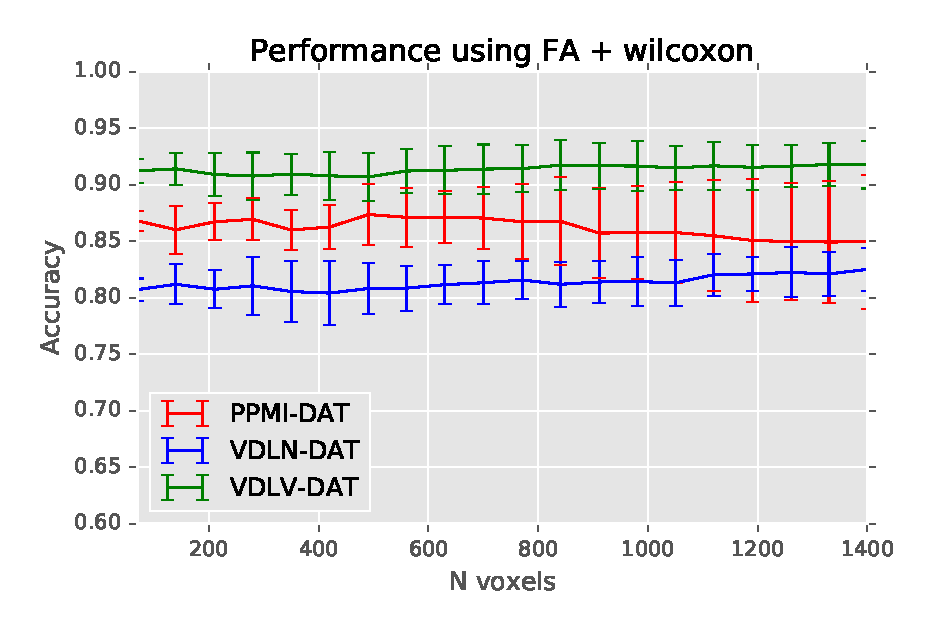
\includegraphics[width=0.49\linewidth]{gfx/ch4/accuracyMeanSTD-FA_vsN_wilcoxon_PKS.eps}\label{fig:PKS-AV-FA-WILCOXON-VSN}}
	\subfloat[]{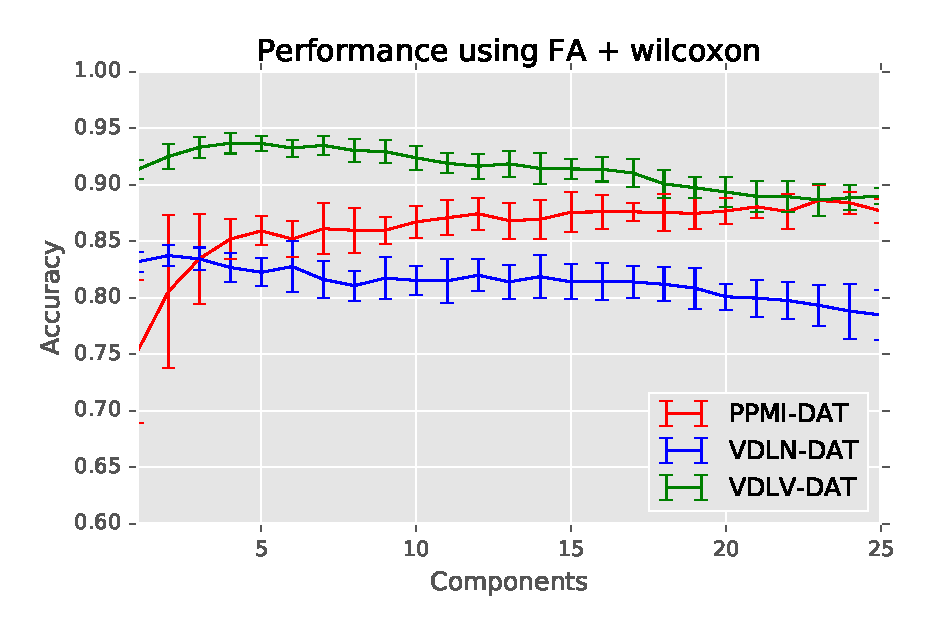
\includegraphics[width=0.49\linewidth]{gfx/ch4/accuracyMeanSTD-FA_vsK_wilcoxon_PKS.eps}\label{fig:PKS-AV-FA-WILCOXON-VSK}}
	
	\caption{Average performance and standard deviation of the proposed system using the three \ac{PKS} datasets, \ac{FA} and the three feature selection criteria: $t$-test (\protect\subref{fig:PKS-AV-FA-TTEST-VSN} and \protect\subref{fig:PKS-AV-FA-TTEST-VSK}), relative entropy (\protect\subref{fig:PKS-AV-FA-ENTROPY-VSN} and \protect\subref{fig:PKS-AV-FA-ENTROPY-VSK}) and wilcoxon (\protect\subref{fig:PKS-AV-FA-WILCOXON-VSN} and \protect\subref{fig:PKS-AV-FA-WILCOXON-VSK}). } 
	\label{fig:accuracyMeanFA-PKS}
\end{bigfigure}

\subsubsection{Independent Component Analysis}
\begin{bigfigure}[-2cm]
	\subfloat[]{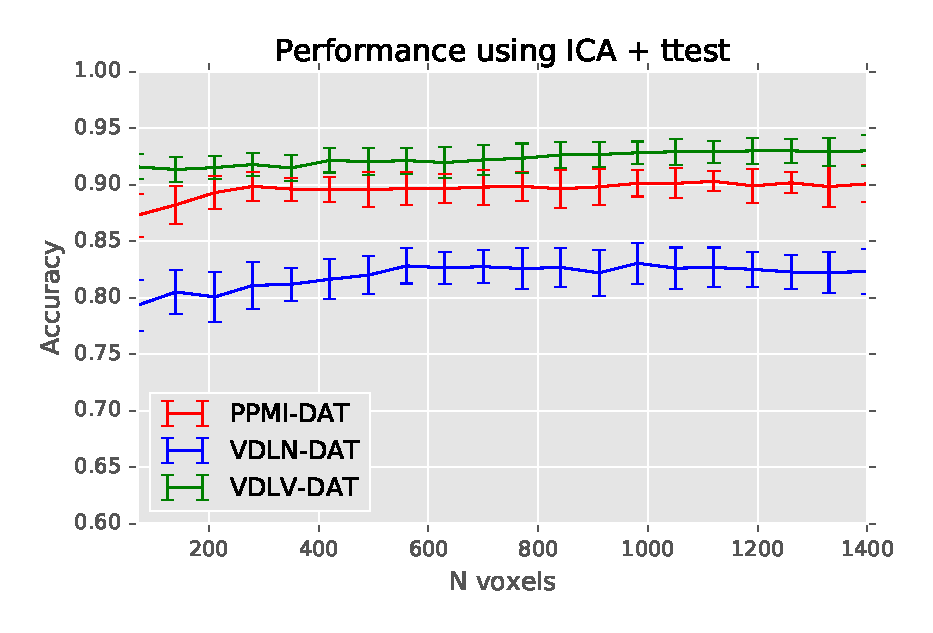
\includegraphics[width=0.49\linewidth]{gfx/ch4/accuracyMeanSTD-ICA_vsN_ttest_PKS.eps}\label{fig:PKS-AV-ICA-TTEST-VSN}}
	\subfloat[]{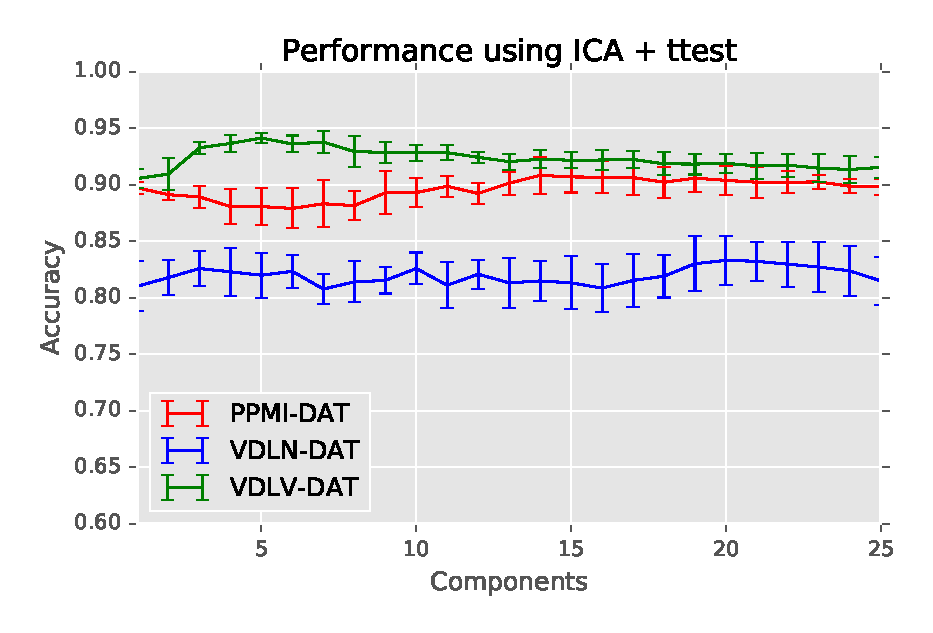
\includegraphics[width=0.49\linewidth]{gfx/ch4/accuracyMeanSTD-ICA_vsK_ttest_PKS.eps}\label{fig:PKS-AV-ICA-TTEST-VSK}}
	
	\subfloat[]{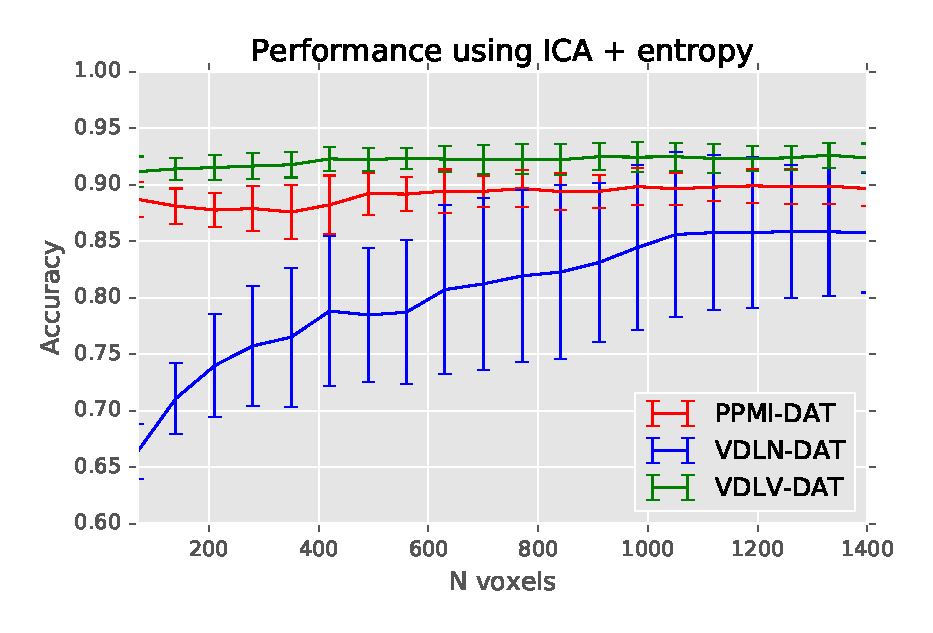
\includegraphics[width=0.49\linewidth]{gfx/ch4/accuracyMeanSTD-ICA_vsN_entropy_PKS.eps}\label{fig:PKS-AV-ICA-ENTROPY-VSN}}
	\subfloat[]{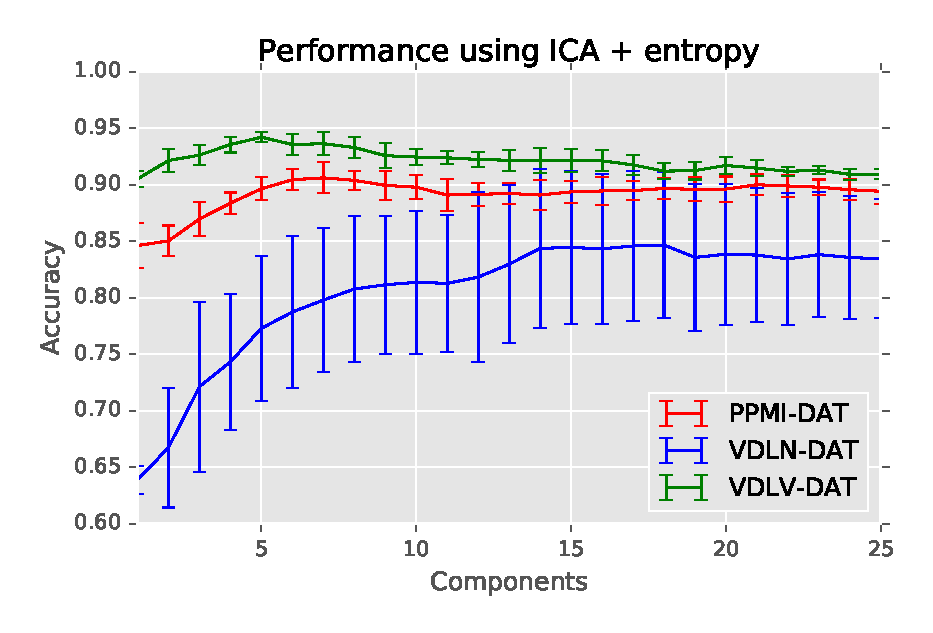
\includegraphics[width=0.49\linewidth]{gfx/ch4/accuracyMeanSTD-ICA_vsK_entropy_PKS.eps}\label{fig:PKS-AV-ICA-ENTROPY-VSK}}
	
	\subfloat[]{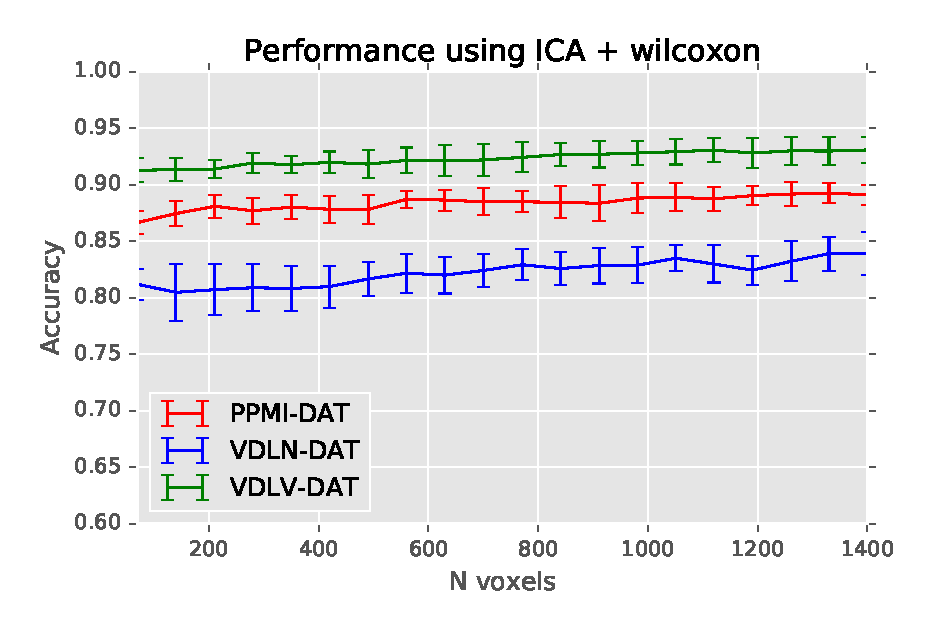
\includegraphics[width=0.49\linewidth]{gfx/ch4/accuracyMeanSTD-ICA_vsN_wilcoxon_PKS.eps}\label{fig:PKS-AV-ICA-WILCOXON-VSN}}
	\subfloat[]{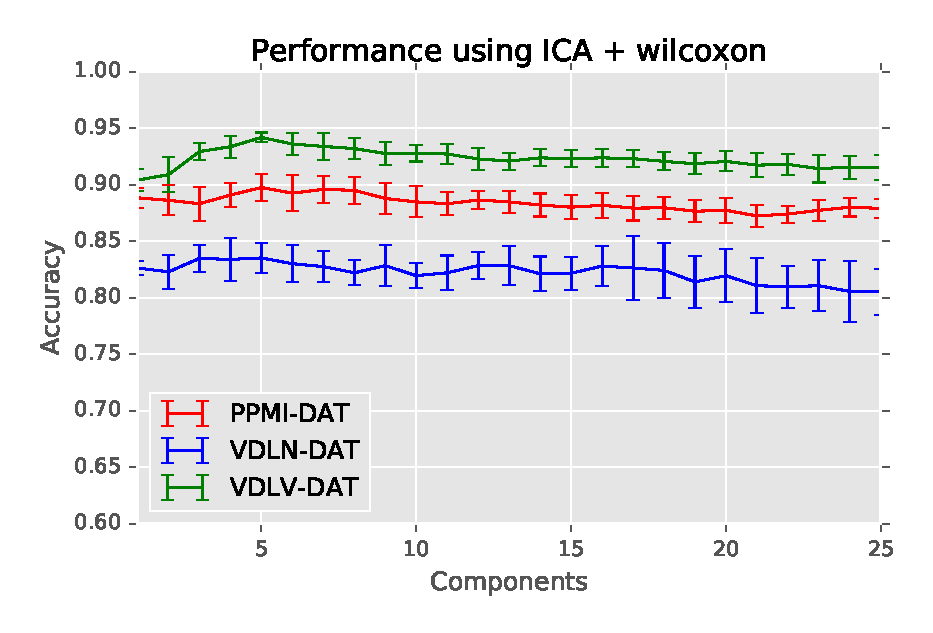
\includegraphics[width=0.49\linewidth]{gfx/ch4/accuracyMeanSTD-ICA_vsK_wilcoxon_PKS.eps}\label{fig:PKS-AV-ICA-WILCOXON-VSK}}
	
	\caption{Average performance and standard deviation of the proposed system using the three \ac{PKS} datasets, \ac{ICA} and the three feature selection criteria: $t$-test (\protect\subref{fig:PKS-AV-ICA-TTEST-VSN} and \protect\subref{fig:PKS-AV-ICA-TTEST-VSK}), relative entropy (\protect\subref{fig:PKS-AV-ICA-ENTROPY-VSN} and \protect\subref{fig:PKS-AV-ICA-ENTROPY-VSK}) and wilcoxon (\protect\subref{fig:PKS-AV-ICA-WILCOXON-VSN} and \protect\subref{fig:PKS-AV-ICA-WILCOXON-VSK}). } 
	\label{fig:accuracyMeanICA-PKS}
\end{bigfigure}


\subsubsection{At the Operation Point}

\begin{bigfigure}[-2cm]
	\subfloat[]{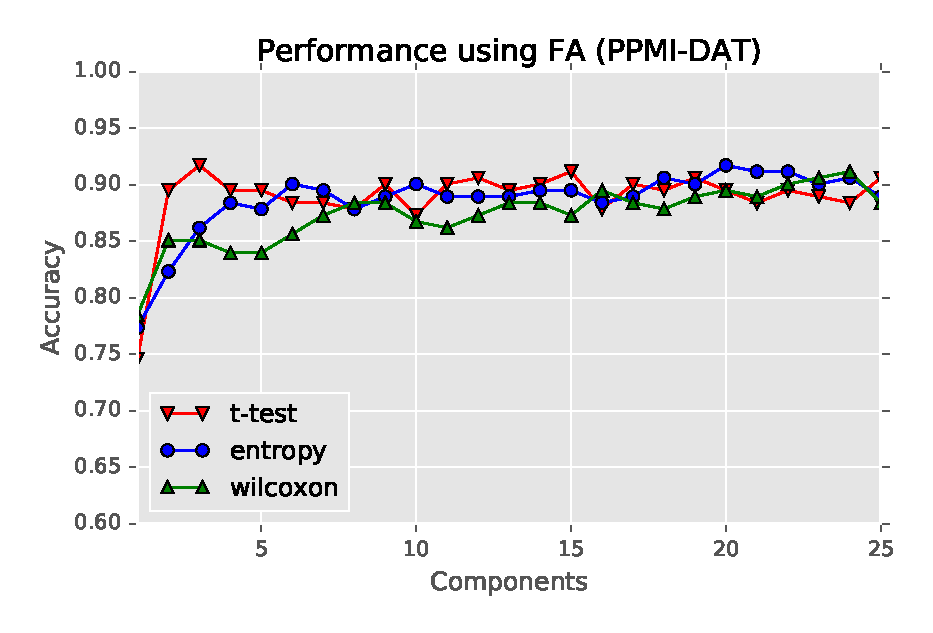
\includegraphics[width=0.49\linewidth]{gfx/ch4/accuracyOP-FA_vsN_comparison_PPMI-DAT.eps}\label{fig:PPMI-DAT-FA-OP}}
	\subfloat[]{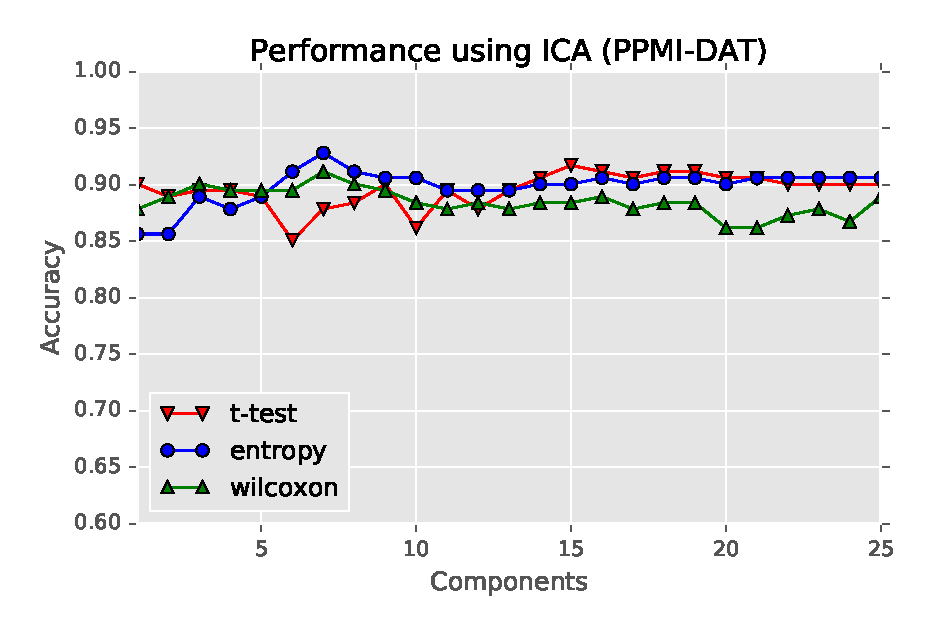
\includegraphics[width=0.49\linewidth]{gfx/ch4/accuracyOP-ICA_vsN_comparison_PPMI-DAT.eps}\label{fig:PPMI-DAT-ICA-OP}}
	
	\subfloat[]{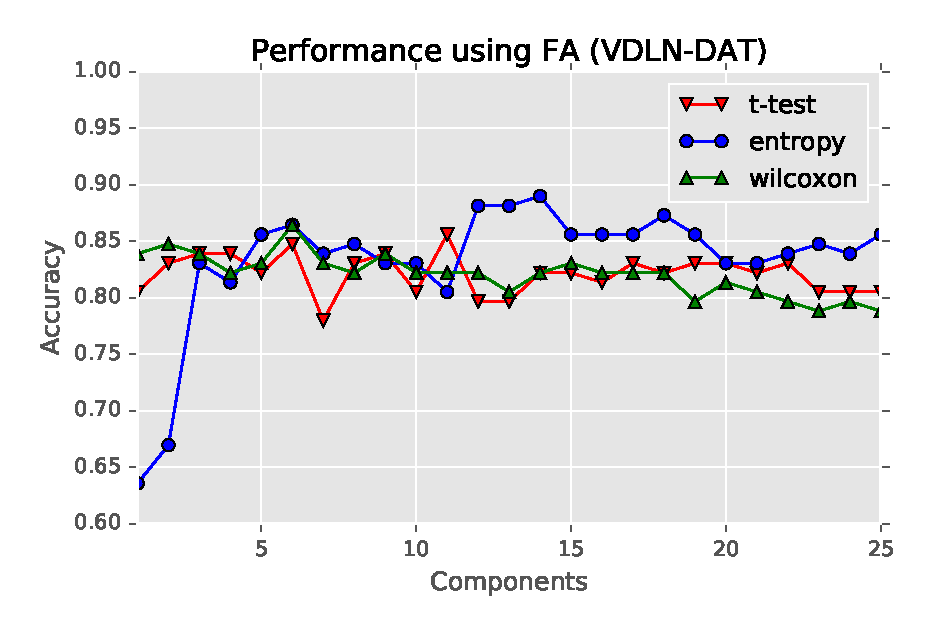
\includegraphics[width=0.49\linewidth]{gfx/ch4/accuracyOP-FA_vsN_comparison_VDLN-DAT.eps}\label{fig:VDLN-DAT-FA-OP}}
	\subfloat[]{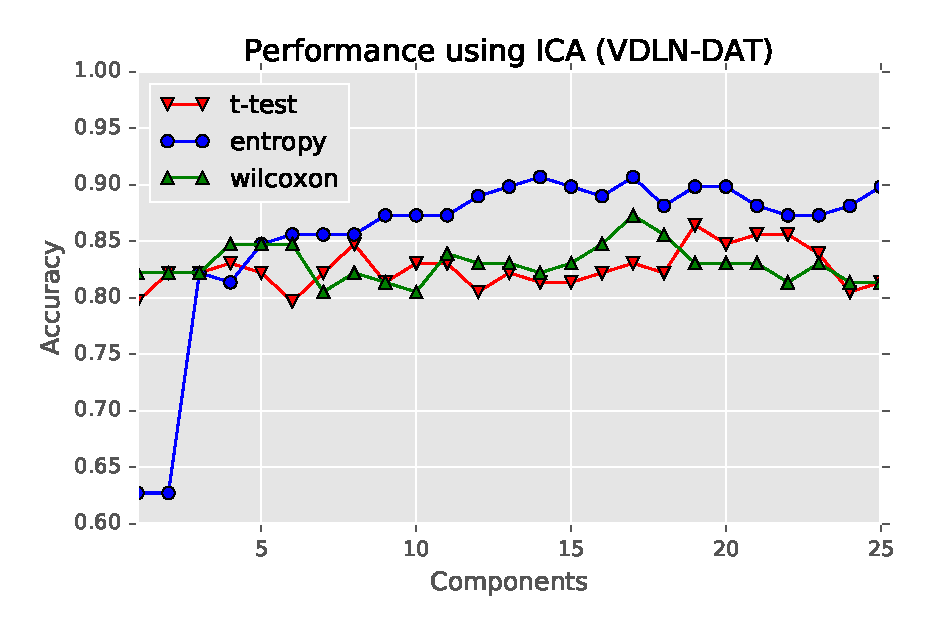
\includegraphics[width=0.49\linewidth]{gfx/ch4/accuracyOP-ICA_vsN_comparison_VDLN-DAT.eps}\label{fig:VDLN-DAT-ICA-OP}}
	
	\subfloat[]{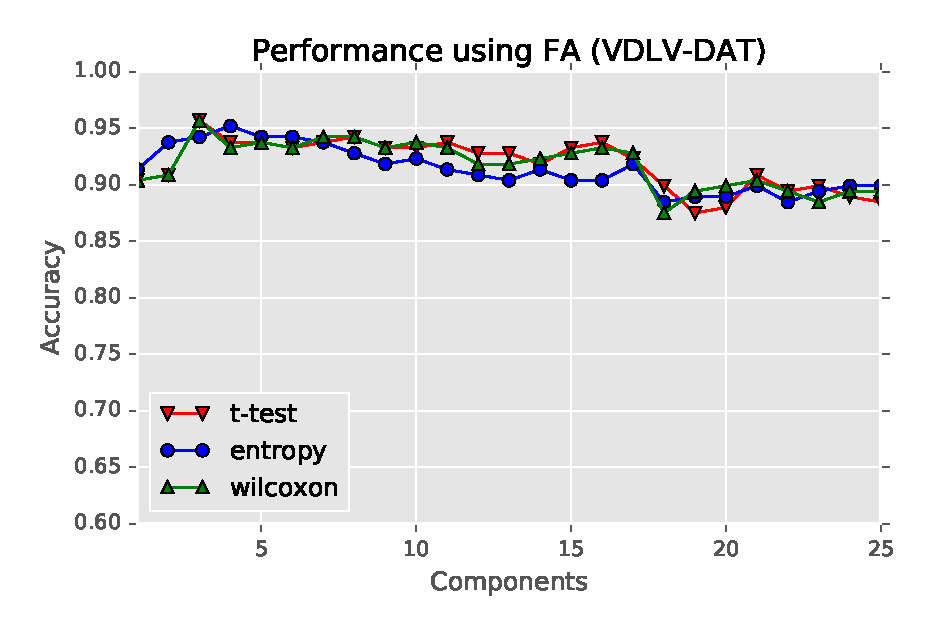
\includegraphics[width=0.49\linewidth]{gfx/ch4/accuracyOP-FA_vsN_comparison_VDLV-DAT.eps}\label{fig:VDLV-DAT-FA-OP}}
	\subfloat[]{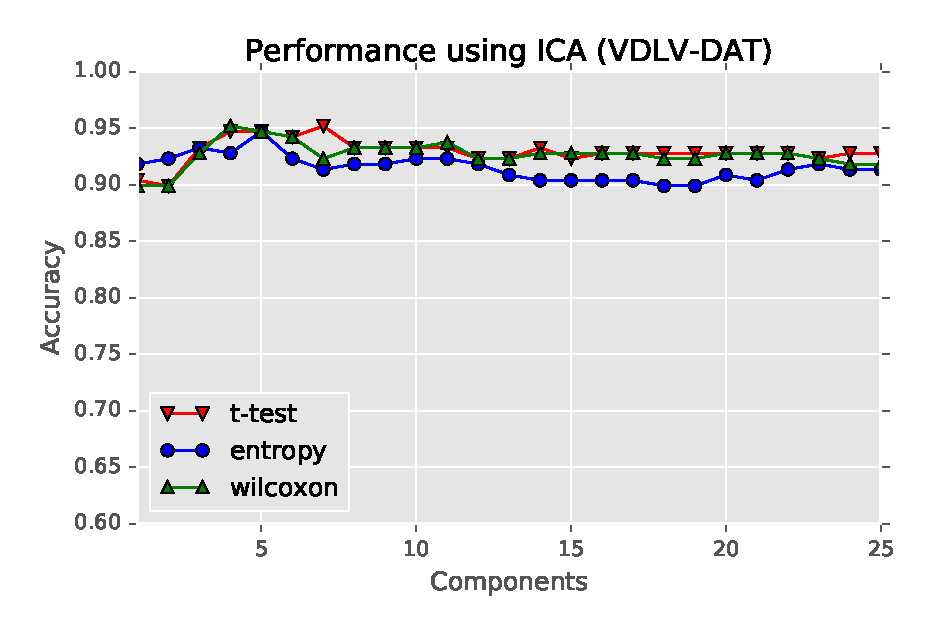
\includegraphics[width=0.49\linewidth]{gfx/ch4/accuracyOP-ICA_vsN_comparison_VDLV-DAT.eps}\label{fig:VDLV-DAT-ICA-OP}}
	
	\caption{Performance of the proposed system using the two \ac{PKS} datasets: PPMI-DAT, VDLN-DAT and VDLV-DAT at the operation point, and how they vary over the number of components used in the decomposition. } 
	\label{fig:accuracyOP-PKS}
\end{bigfigure}


\begin{bigtable}[-2cm]
	\begin{tabularx}{\linewidth}{Xllccc}
		\tableheadline{DB} & \tableheadline{Dec.} & \tableheadline{Criterion} & \tableheadline{Accuracy} & \tableheadline{Sensitivity} & \tableheadline{Specificity}\\
		\toprule
		\multirow{6}{1.7cm}{VDLN-DAT} & \multirow{3}{*}{\ac{FA}} & t-test & $ 0.856 \pm 0.111 $ & $ 0.887 \pm 0.178 $ & $ 0.795 \pm 0.164 $ \\
		&  & entropy & $ 0.890 \pm 0.098 $ & $ 0.875 \pm 0.118 $ & $ 0.910 \pm 0.116 $ \\
		&  & wilcoxon & $ 0.864 \pm 0.070 $ & $ 0.916 \pm 0.114 $ & $ 0.780 \pm 0.183 $ \\
		\cline{2-6}
		& \multirow{3}{*}{\ac{ICA}} & t-test & $ 0.864 \pm 0.101 $ & $ 0.873 \pm 0.174 $ & $ 0.840 \pm 0.166 $ \\
		&  & entropy & $ 0.907 \pm 0.075 $ & $ 0.889 \pm 0.124 $ & $ 0.935 \pm 0.131 $ \\
		&  & wilcoxon & $ 0.873 \pm 0.108 $ & $ 0.859 \pm 0.181 $ & $ 0.890 \pm 0.151 $ \\
		\midrule
		\multirow{6}{1.7cm}{VDLV-DAT} & \multirow{3}{*}{\ac{FA}} & t-test & $ 0.957 \pm 0.033 $ & $ 0.940 \pm 0.066 $ & $ 0.973 \pm 0.065 $ \\
		&  & entropy & $ 0.952 \pm 0.037 $ & $ 0.940 \pm 0.066 $ & $ 0.964 \pm 0.064 $ \\
		&  & wilcoxon & $ 0.957 \pm 0.033 $ & $ 0.940 \pm 0.066 $ & $ 0.973 \pm 0.065 $ \\
		\cline{2-6}
		& \multirow{3}{*}{\ac{ICA}} & t-test & $ 0.952 \pm 0.037 $ & $ 0.940 \pm 0.066 $ & $ 0.964 \pm 0.064 $ \\
		&  & entropy & $ 0.947 \pm 0.045 $ & $ 0.940 \pm 0.066 $ & $ 0.955 \pm 0.076 $ \\
		&  & wilcoxon & $ 0.952 \pm 0.037 $ & $ 0.940 \pm 0.066 $ & $ 0.964 \pm 0.064 $ \\
		\midrule
		\multirow{6}{1.7cm}{PPMI-DAT} & \multirow{3}{*}{\ac{FA}} & t-test & $ 0.917 \pm 0.037 $ & $ 0.918 \pm 0.095 $ & $ 0.918 \pm 0.091 $ \\
		&  & entropy & $ 0.917 \pm 0.060 $ & $ 0.918 \pm 0.076 $ & $ 0.921 \pm 0.120 $ \\
		&  & wilcoxon & $ 0.912 \pm 0.056 $ & $ 0.927 \pm 0.098 $ & $ 0.889 \pm 0.102 $ \\
		\cline{2-6}
		& \multirow{3}{*}{\ac{ICA}} & t-test & $ 0.917 \pm 0.056 $ & $ 0.900 \pm 0.095 $ & $ 0.948 \pm 0.109 $ \\
		&  & entropy & $ 0.928 \pm 0.055 $ & $ 0.909 \pm 0.091 $ & $ 0.961 \pm 0.090 $ \\
		&  & wilcoxon & $ 0.912 \pm 0.070 $ & $ 0.909 \pm 0.100 $ & $ 0.920 \pm 0.118 $ \\
		\bottomrule
		\end{tabularx}
		\caption{Accuracy, sensitivity, specificity, and their standard deviation at the operation point for each method and its corresponding feature selection criterion, using three \protect\ac{PKS} datasets }
		\label{tab:featurePKS}
\end{bigtable}

\section{Discussion}